
\documentclass[10pt,english]{article}
\usepackage{ae}
\usepackage{aecompl}
\usepackage[T1]{fontenc}
\usepackage{ucs}
\usepackage[utf8x]{inputenc}
\usepackage{babel}
\usepackage{geometry}
\geometry{a4paper,tmargin=3cm,bmargin=3cm,lmargin=2.5cm,rmargin=2.5cm,headsep=1cm}
\usepackage{graphicx}
\usepackage{color}
\usepackage{array}
\usepackage[dvips, bookmarks, bookmarksopen=true, bookmarksopenlevel=2, colorlinks=true, pdfview=FitH, pdfstartview=FitH, urlcolor=blue, linkcolor=black, pdftitle={Aqualung User's Manual}]{hyperref}
\usepackage{fancyhdr}
\pagestyle{fancy}
\sloppy
\lhead{Aqualung User's Manual}
\chead{}
\rhead{\thepage}
\lfoot{}
\cfoot{}
\rfoot{}
\begin{document}
\begin{titlepage}
\begin{center}
\hspace{0mm}
\vspace{10mm}\\
{\Huge\bf Aqualung}
\vspace{3mm}\\
{\LARGE Music Player for GNU/Linux}
\vspace{10mm}\\
\today
\vspace{70mm}\\
{\Huge User's Manual}
\vspace{60mm}\\
Copyright \copyright{} 2006-2010 Peter Szilagyi
\vspace{5mm}\\
Permission is granted to copy, distribute and/or modify this document\\
under the terms of the GNU Free Documentation License, Version 1.2\\
or any later version published by the Free Software Foundation.
\end{center}
\end{titlepage}
\tableofcontents{}
\newpage{}


\section{Introduction\label{idp281392}}



\noindent Aqualung is an advanced music player originally targeted at
the GNU/Linux operating system, today also running on FreeBSD,
OpenBSD and Microsoft Windows. It plays audio CDs, internet
radio streams and podcasts as well as soundfiles in just about
any audio format and has the feature of inserting \emph{no
gaps} between adjacent tracks. It also supports high
quality sample rate conversion between the file and the output
device, when necessary.




Audio CDs can be played back and ripped with on-the-fly
conversion to WAV, FLAC, Ogg Vorbis or CBR/VBR MP3 (gapless via
LAME). Seamless tagging of the created files is offered as part
of the process. Internet radio stations streaming Ogg Vorbis or
MP3 are supported. Subscribing to RSS and Atom audio podcasts is
supported: Aqualung can automatically download and add new files
to the Music Store. Optional limits for the age, size and number
of downloaded files can be set.




Almost all sample-based, uncompressed formats (e.g. WAV,
AIFF, AU etc.), as well as files encoded with FLAC (the Free
Lossless Audio Codec), Ogg Vorbis, Ogg Speex, MPEG Audio
(including the infamous MP3 format), MOD audio formats (MOD,
S3M, XM, IT, etc.), Musepack and Monkey's Audio Codec are
supported. Numerous formats and codecs are also supported via
the FFmpeg project, including AC3, AAC, WMA, WavPack and the
soundtrack of many video formats. There is also a native
(non-FFmpeg) WavPack decoder. The program can play the music
through OSS, ALSA, sndio, PulseAudio, the JACK Audio Connection
Kit, or even using the Win32 Sound API (available only under
Cygwin or native Win32). Depending on the compile-time options,
not all file formats and output drivers may be usable in a
particular build. Type \texttt{aqualung -v} to get a list of
all the compiled-in features.




Aqualung supports the LADSPA 1.1 plugin standard. You can use
any suitable plugin to enhance the music you are listening
to.




Other features of the program are: tabbed playlist,
internally working volume and balance controls (not touching the
soundcard mixer), multiple skin support, random seeking during
playback, track repeat, list repeat and shuffle mode (besides
normal playback). In track repeat mode the looping range is
adjustable. Aqualung will come up in the same state as it was
when you closed it, including playback modes, volume and balance
settings, currently processing LADSPA plugins, window sizes,
positions and visibility, and other miscellaneous
options. Aqualung has the ability to display and edit Ogg Xiph
comments, ID3v1, ID3v2 and APE tags, as well as FLAC picture
frames found in files that support them. See the section about
\hyperref[idp695360]{\color{blue}metadata support} for full reference.




The method of assembling the title string of a track is programmable
(via a user-provided Lua function) and can include nearly any metadata
item or audio file attribute. See the documentation of the
\hyperref[idp808416]{\color{blue}\textsl{Lua extension file}
config setting} for full reference.




You can control any running instance of the program remotely
from the command line (start, stop, pause etc.). Remote loading
or enqueueing soundfiles as well as complete playlists is also
supported.




In addition to all this, Aqualung provides a so-called Music
Store that is an XML-based music database, capable of storing
various metadata about music on your computer (including, but
not limited to, the names of artists, and the titles of records
and tracks). You can (and should) organize your music into trees
of Artists/Records/Tracks, thereby making life easier than with
the all-in-one Winamp/XMMS playlist. Importing file metadata
(ID3v1, ID3v2 tags, Ogg Xiph comments, APE metadata) into the
Music Store as well as getting track names from a CDDB/FreeDB
database is supported. For audio CDs, CD-Text retrieval is also
implemented.




\section{Quick Start Guide\label{idp320880}}



\noindent If you'd like to get your hands on the program quickly rather
than to spend your evening reading the rest of the manual, here
is the absolute minimum you need to know to successfully use the
program. So make sure to read this (deliberately short) chapter,
and come back for the rest when you have questions while using
the program. Ultimately, you may ask questions on the
\href{https://lists.sourceforge.net/lists/listinfo/aqualung-friends}{
aqualung-friends
\includegraphics[scale=0.5]{external.eps}} mailing list.


\subsection{Getting Aqualung\label{idp322992}}



\noindent It is not hard to get Aqualung up and running on your
machine, although for beginners the number of compile-time
options might be intimidating at first. The steps you need to
take depend on the platform and operating system you use. For
detailed information please look at the \href{http://aqualung.factorial.hu/compiling.html}{relevant
page
\includegraphics[scale=0.5]{external.eps}} of the Aqualung website.




In case you are not used to compiling software yourself,
you may check whether there is a distribution-provided package
of Aqualung. Installing such a package is generally the
easiest and fastest way to get Aqualung, however this way you
won't be able to try the latest features. Currently there are
Aqualung packages for major Linux distributions such as \href{http://packages.debian.org/aqualung}{Debian
\includegraphics[scale=0.5]{external.eps}}, Gentoo,
SuSE, etc. as well as \href{http://www.freshports.org/audio/aqualung}{
FreeBSD
\includegraphics[scale=0.5]{external.eps}}. If your distribution lacks such a package,
consider contacting the organization maintaining the
distribution and ask them to provide a package of
Aqualung. Anyway, you might have to compile Aqualung from
source. This is not very hard, either -- the
\texttt{configure} script tries to adapt Aqualung to your
system as much as possible without breaking the program. See
the above website for more information.




On Microsoft Windows, all you have to do is download and
run the self-extracting installer utility, which guides you
through a few easy to follow steps and installs the program on
your machine. Make sure to visit \href{http://aqualung.factorial.hu/win32}{this page
\includegraphics[scale=0.5]{external.eps}} for
more information about the Windows version of Aqualung.




\subsection{Starting the program for the first time\label{idp329856}}



\noindent Aqualung has a large number of configuration settings,
which are adjustable through the user interface at run-time
(no need to edit config files by hand), and are remembered
across multiple invocations of the program. When Aqualung
starts for the first time, it creates a configuration based on
some wired-in defaults. A good way of exploring the program's
capabilities is poking through the configuration area. You can
access this by clicking in the main window with the right
mouse button, which will pop up the program's main
menu. Choosing \textsl{Settings} from the menu will open the
configuration dialog.




In fact, clicking with the right mouse button almost
anywhere is a generally smart idea. Aqualung has lots of
context-sensitive popup menus in the Music Store, the Playlist
(often embedded in the main window) and elsewhere. It's good
to keep this in mind when taking the explorative approach
instead of reading the whole manual right away.




Let's add some music to the Playlist and start playback
right away. Right-click the \textsl{Add files} button, and
choose \textsl{Add directory} from the menu. (The
right-clicking trick works for the other two buttons as
well. Left-clicking is a shortcut to immediately execute the
action denoted by the button's caption.) Choose a directory
with some music under it. It's OK to have subdirectories under
this directory, the program will search for playable files
recursively. After the Playlist starts to get populated with
tracks, press play, or double-click on one of the tracks to
play. Press `i' to see metadata information about the
selected track.




\subsection{Setting up a Music Store\label{idp335856}}



\noindent Now that you have some music playing, let's get more
organized. In the Music Store window click in the empty area
with the right mouse button and choose \textsl{Create empty
store\dots{}} from the menu. Enter a meaningful name such as
`Tom's Music' and choose a location to save the XML file
of the store to. This should be a writable location, so it is
wise to stick to a location inside your home directory. (A
system-wide path or a remote NFS mount with read-only access
won't do.)




You can have any number of such stores in the Music Store
organizer, and it is indeed a great idea to have separate
stores for music differentiated by origin, genre, or some
other aspect. One great use is multiple stores with the actual
music files stored on multiple remote machines, one store for
each machine. Or just a store for your local music and another
for files on your bedroom file server box. There are several
possibilities.




But how do you populate the store with music you already
have on your drive? It's easy if your music is stored in an
organized manner on the filesystem level. As a minimum, this
means that tracks intended to go into one store are found
under a common root directory in the filesystem (there may be
several directory layers down from the root to the individual
files, but there must be a common ancestor). In this case the
so-called Music Store Builder will take care of things for
you. Right-click on your newly-created empty store and choose
\textsl{Build / Update store from filesystem}. Choose
Independent mode and in the dialog you get, enter the root
directory under which your collection resides. As you can
probably guess at this point, the store builder interface is
pretty flexible, however the default settings should be good
to get something together quickly without further hassle.




Pressing \textsl{OK} will start the process, during which
the directory structure below the root you specified will be
traversed. The artist/record/track names are determined from
potentially multiple data sources (CDDB, metadata e.g. ID3v2
tags or Ogg Xiph comments, and filesystem names). The logic
involved is fairly elaborate. You are strongly advised to \hyperref[idp663728]{\color{blue}read} the detailed usage instructions
for the Music Store Builder.




\subsection{Playing and ripping an Audio CD\label{idp343536}}



\noindent You can play CDs with Aqualung easily. Just put the CD in
one of your CD drives, and if everything goes well, Aqualung
will detect it, do a CDDB lookup to retrieve artist, record
and track info (CD-Text is also used if the CD has it), and
make it available to you through the special Music Store node
called `CD Audio'.




You don't have to be happy with what you have so far. The
Music Store paradigm is fairly addictive, as it's much easier
to drop something into the Playlist from the Music Store than
physically placing a CD in the drive. So as you keep expanding
your CD collection, you will probably want to have those
records in one of your music stores, too. In this case all you
have to do is choose \textsl{Rip CD\dots{}} from the disc's
popup menu, and supply some information. We won't go into
details here (please refer to \hyperref[idp589520]{\color{blue}this
section} in case the interface is not obvious). However,
it is worth stating that you should have a separate directory
for the files of each record. Ripping multiple CDs into the
same directory won't work.






\section{Command Line Interface\label{idp347968}}

\subsection{Invocation\label{idp348496}}

\begin{description}

\item [
\texttt{aqualung {-}{-}help}
]

Print help message with valid parameters and
example invocations.

\item [
\texttt{aqualung {-}{-}version}
]

Print version information and list of
compiled-in features.

\item [
\texttt{aqualung [{-}{-}output (jack|pulse|alsa|oss|sndio|win32)] [options] [file1 [file2 \dots{}]]}
]

\end{description}



\noindent Normally you should be able to start Aqualung
without any options. This case the output device will be
selected by probing for a usable driver (in order of JACK,
PulseAudio, ALSA, OSS) with default parameters.




If no driver could be started with default
parameters, or you want to explicitly choose a suitable output
configuration, you have to tell the program which output
device to use. This is possible with the \texttt{-o}
(\texttt{{-}{-}output}) option. There are specific optional
parameters for all five output drivers. You can also specify
which sample rate converter you want to use, or request a list
of available converters. You may also control another instance
of the program remotely, or add files to the Playlist.




\subsection{General options\label{idp356752}}

\begin{description}

\item [
\texttt{-D, {-}{-}disk-realtime}
]

Try to use realtime (\texttt{SCHED\_FIFO}) scheduling
for disk thread, a background worker thread doing file
decoding and sample rate conversion. Try this (and
optionally \texttt{-Y}) if you experience short audio
dropouts caused by other programs (e.g. web browser loading
a complex page).

\item [
\texttt{-Y, {-}{-}disk-priority <int>}
]

When running \texttt{-D}, set scheduler priority to
<int> (defaults to 1).

\end{description}



\subsection{Output specific options\label{idp362208}}

\subsubsection{Options relevant to ALSA output\label{idp362736}}

\begin{description}

\item [
\texttt{-d, {-}{-}device <name>}
]

Set the output device (defaults to 'default').

\item [
\texttt{-r, {-}{-}rate <int>}
]

Set the output sample rate.

\item [
\texttt{-b, {-}{-}buffer-size <int>}
]

Set the ALSA output buffer size (in frames).

\item [
\texttt{-R, {-}{-}realtime}
]

Try to use realtime (\texttt{SCHED\_FIFO}) scheduling
for ALSA output thread.

\item [
\texttt{-P, {-}{-}priority <int>}
]

When running \texttt{{-}{-}realtime}, set scheduler
priority to <int> (default is 1 when -R is used).

\end{description}



\subsubsection{Options relevant to OSS output\label{idp389104}}

\begin{description}

\item [
\texttt{-d, {-}{-}device <name>}
]

Set the output device (defaults to
\texttt{/dev/audio} on OpenBSD, \texttt{/dev/dsp}
on other Unices).

\item [
\texttt{-r, {-}{-}rate <int>}
]

Set the output sample rate.

\item [
\texttt{-R, {-}{-}realtime}
]

Try to use realtime (\texttt{SCHED\_FIFO}) scheduling
for OSS output thread.

\item [
\texttt{-P, {-}{-}priority <int>}
]

When running \texttt{{-}{-}realtime}, set scheduler
priority to <int> (default is 1 when -R is used).

\end{description}



\subsubsection{Options relevant to JACK output\label{idp396800}}

\begin{description}

\item [
\texttt{-a[<port\_L>,<port\_R>],
{-}{-}auto[=<port\_L>,<port\_R>]}
]

Auto-connect output ports to given JACK ports
(defaults to first two hardware playback ports).

\item [
\texttt{-c, {-}{-}client <name>}
]

Set client name (needed if you want to run multiple
instances of the program).

\end{description}



\noindent Note that in the case when JACK output has been selected
as part of the automatic output device detection, the
\texttt{-a} option is implicitly applied.




\subsubsection{Options relevant to PulseAudio and sndio output\label{idp401808}}

\begin{description}

\item [
\texttt{-r, {-}{-}rate <int>}
]

Set the output sample rate.

\item [
\texttt{-R, {-}{-}realtime}
]

Try to use realtime (\texttt{SCHED\_FIFO}) scheduling
for sndio output thread.

\item [
\texttt{-P, {-}{-}priority <int>}
]

When running \texttt{{-}{-}realtime}, set scheduler
priority to <int> (default is 1 when -R is used).

\end{description}



\subsubsection{Options relevant to Win32 output\label{idp407840}}

\begin{description}

\item [
\texttt{-r, {-}{-}rate <int>}
]

Set the output sample rate.

\end{description}





\subsection{Options relevant to the Sample Rate Converter\label{idp410544}}

\begin{description}

\item [
\texttt{-s[<int>], {-}{-}srctype[=<int>]}
]

Choose the SRC type, or print the list of available
types if no number given. The default is SRC type 4 (Linear
Interpolator).

\end{description}



\subsection{Options for remote cue control\label{idp413264}}



\noindent Note that remote controlling of instances is only possible
if the instance you want to send a command to is running as
the same user as you are when you issue the remote command.


\begin{description}

\item [
\texttt{-N, {-}{-}session <int>}
]

Specify the instance number to send the remote command
to. Instances are numbered on a per user basis, starting
with 0. Except for the zero-th instance (started first), the
instance number is displayed in the title bar of the main
window (e.g.: `Aqualung.3'). If you don't use this
option, the following options will control the zero-th
instance by default, except for \texttt{-L} which defaults
to the present instance (so as to be able to start playback
immediately from the command line).

\item [
\texttt{-B, {-}{-}back}
]

Jump to previous track.

\item [
\texttt{-F, {-}{-}fwd}
]

Jump to next track.

\item [
\texttt{-L, {-}{-}play}
]

Start playing.

\item [
\texttt{-U, {-}{-}pause}
]

Pause playback, or resume if already paused.

\item [
\texttt{-T, {-}{-}stop}
]

Stop playback.

\item [
\texttt{-V, {-}{-}volume [m|M]|[=]<val>}
]

Adjust the volume. \texttt{m/M} means
mute; if \texttt{=} is present, the remote instance's
volume control will be set to the value specified,
otherwise, the volume will be adjusted by the supplied
(signed) value. The values are in dB units.

\item [
\texttt{-Q, {-}{-}quit}
]

Terminate remote instance.

\end{description}




\subsection{Options for file loading\label{idp427552}}



\noindent You may specify filenames on the command line. These may be
ordinary soundfiles playable by Aqualung, directories, or
playlist files you saved earlier. The program will decide if a
file is a playlist, and add its contents accordingly. In
addition to Aqualung's native (XML) playlist format, the
program will load M3U and PLS playlists whenever possible.




If you used the \texttt{{-}{-}session} option (see above),
the files will be sent to the Aqualung instance you
specified. Otherwise a new instance will start up with the
files you specified. Note that if you enabled the \textsl{Save
and restore the Playlist on exit/startup} option in the
\textsl{Settings} dialog, the files you specify will be
loaded \emph{after} the automatically loaded ones.


\begin{description}

\item [
\texttt{-E, {-}{-}enqueue}
]

Enqueue added files to the Playlist instead of loading
them (which removes the previous contents of the
Playlist). Use this if you want to keep the existing items
in the Playlist.

\item [
\texttt{-t[<name>], {-}{-}tab[=<name>]}
]

Specify target tab for file loading (either remotely
using the \texttt{{-}{-}session} option, or at startup). If
\texttt{{-}{-}tab} is used without the name parameter, the
files will be added to a new (untitled) tab. If a name is
supplied, Aqualung will check whether a tab with that name
already exists. If so, the files will be loaded (or enqueued
if you used \texttt{-E}) to that tab. If no such tab
exists, one with that name will be created, and the content
goes there.

\end{description}

\subsubsection{Setting up programs to use Aqualung as a soundfile handler\label{idp436480}}



\noindent It is possible to set up a host program such as a
browser, file manager etc. to use Aqualung for opening
soundfiles. To do this, a command line with the following
properties should be used:


\begin{itemize}
\item if an Aqualung instance is already running, send the file(s) to that instance;
\item if no instance is running, start up a new instance;
\item either case, start playing the file(s) immediately after loading them.
\end{itemize}



\noindent One solution to this is to use


\begin{description}

\item [\texttt{aqualung -N0 -E -L -t'File Manager' \%s}]
\end{description}



\noindent where \texttt{\%s} is one or more filenames. It should be noted
that the file associations (the mechanism of knowing which
files to open via Aqualung) is completely within the scope
of the host program.






\subsection{Options for changing state of Playlist/Music Store windows\label{idp442608}}

\begin{description}

\item [
\texttt{-l [yes|no], {-}{-}show-pl=[yes|no]}
]

Show/hide Playlist window.

\item [
\texttt{-m [yes|no], {-}{-}show-ms=[yes|no]}
]

Show/hide Music Store window.

\end{description}



\subsection{Examples\label{idp446464}}

\begin{description}

\item [
\texttt{\$ aqualung -s3 -o alsa -R -r 48000 -d plughw:0,0}
]

\item [
\texttt{\$ aqualung {-}{-}srctype=1 {-}{-}output oss {-}{-}rate 96000}
]

\item [
\texttt{\$ aqualung -o jack {-}{-}auto=system:playback\_17,system:playback\_18}
]

\item [
\texttt{\$ aqualung -o jack -a -E {-}{-}tab="Led Zeppelin" `find ./ledzeppelin/ -name '*.flac'`}
]

\end{description}




\subsection{Environment\label{idp451152}}



\noindent Aqualung obeys two environment variables
concerning LADSPA plugins.


\begin{description}

\item [
\texttt{LADSPA\_PATH}
]

Colon-separated list of paths to search for LADSPA
plugin \texttt{.so} files.

\item [
\texttt{LADSPA\_RDF\_PATH}
]

Colon-separated list of paths to RDF metadata files
about these plugins.

\end{description}



\noindent When any of these is not specified, the
program will use sensible defaults and look in the obvious
places.




\subsection{Files\label{idp456976}}



\noindent Here is a list of files that Aqualung creates, reads and
relies on.


\begin{description}

\item [
\texttt{\textasciitilde{}/.aqualung}
]

Directory containing user settings.

\item [
\texttt{\textasciitilde{}/.aqualung/config.xml}
]

GUI (skin, window size/position, etc.) and other
settings.

\item [
\texttt{\textasciitilde{}/.aqualung/plugin.xml}
]

List of running plugins and all their settings.

\item [
\texttt{\textasciitilde{}/.aqualung/playlist.xml}
]

Automatically saved and restored playlist (if you enable
this feature).

\item [
\texttt{\textasciitilde{}/.aqualung/<skin-name>}
]

Locally available skin <skin-name> (useful for
skin development).

\item [
\texttt{\$\{prefix\}/share/aqualung/skin}
]

System-wide skin directory.

\end{description}





\section{Graphical Interface\label{idp466848}}

\subsection{Main Window\label{idp467376}}



\noindent You can control most of the program from this window. The
cue controls in the bottom-left corner are fairly obvious. You
can drag the large slider in the middle for seeking. There are
two smaller sliders above that, the left one is for adjusting
the volume and the right one for adjusting the balance. Above
these, there are two horizontal text areas showing information
about the currently playing track, and input/output parameters
such as sample rate, mono/stereo, bitrate, output driver
(e.g. OSS, ALSA, JACK) etc. The first trick to learn is that
these lines are horizontally draggable with the mouse if the
text does not fit in the available visible space. However,
they don't scroll automatically, and for a very good reason.




In the upper left corner, you find one bigger and two
smaller displays that show track times: elapsed time,
remaining time and total track time. The big display also
shows the current volume and balance setting when
appropriate. By clicking in these displays, you can rearrange
the displays as you want them. The following figure shows how
the displays switch their contents after clicking into them
with the left (L) or right (R) mouse button.


\begin{figure}[h!] \centering 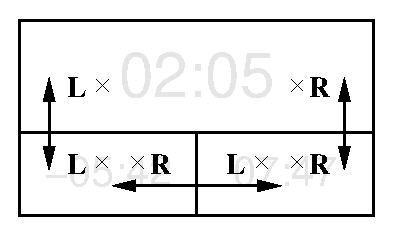
\includegraphics[scale=0.7]{timer.eps}\end{figure}



\noindent In the bottom right corner there are additional
buttons. The buttons with the letters display or hide
additional windows of the program:


\begin{center}\begin{tabular}{|l|l|}\hline 

FX&
Ladspa Patch Builder
\\ \hline 

MS&
Music Store
\\ \hline 

PL&
Playlist
\\ \hline 
\end{tabular}\end{center}



\noindent Note that depending on the skin, these buttons may come
with images instead of the letters above. However, their
functionality does not change.




The remaining three buttons are to select the playback
mode. When none of these buttons is depressed, playback goes
the normal way. The buttons are mutually exclusive, and select
track repeat, list repeat or shuffle mode. I'm sure you can
figure out which is which. If you select track repeat, a loop
bar appears above the seek bar, with two markers. The markers
can be dragged to select the looping range. When they are at
the left and right end positions, the whole song is repeated.
The looping range can also be selected using keyboard
shortcuts. When track repeat is enabled and the current song
is playing (or paused), `<' will set the start of the
looping range to the current playing position; `>' does
the same for the end of the looping range.




Volume and balance slider tricks:


\begin{itemize}
\item Shift + any mouse button sets the volume and balance
sliders back to 0 dB and Center position, respectively. This
combination also works for the loop bar, in which case the
looping range is set to the whole song.

\item Clicking and holding the right mouse button on these
sliders shows their position in the big time display without
altering the value.
\end{itemize}



\noindent An additional thing to know about the volume control is
that it ranges up to +6 dB. This means you can send a bigger
signal to the audio device than in the original file. With 0
dB corresponding to 100\% signal level, +6 dB is almost exactly
200\% signal level (and 4 times signal power as well). This
means you can overdrive your output device, and since clipping
will occur at 100\% anyway, it will cause nasty digital
distortion much worse than simple analog overdrive. If you
have a track with a reasonably low level, you can go above 0
dB with the volume control. But today most CDs are mastered to
keep the average volume level very close to the 0 dB (or 100\%)
top, and so they will likely distort with as little as +1 dB
additional gain. The moral is: if you want it loud, turn up
your external amp. You can also consider using RVA if the
volume level of your tracks tends to vary in a wide range
-- see \hyperref[idp645824]{\color{blue}this section} for
details.




On a related note, another thing to watch out for is LADSPA
plugins (in case you use them). It is very common that the
signal level leaving a plugin is greater than the signal level
the plugin gets on its input. So it is best to leave a few dB
of headroom if you do that. A very typical case is boosting
some frequency bands a few dB with an EQ plugin. You should
decrease the overall volume level with as much dB as the
largest boost (or even more), or you are risking that the
signal will get chopped causing bad distortion. Alternatively,
apply \href{http://tap-plugins.sourceforge.net/ladspa/limiter.html}{this
limiter plugin
\includegraphics[scale=0.5]{external.eps}} as the last one in the processing chain,
but only if you know what you are doing.




Right-clicking almost anywhere in the window will bring up
a menu that allows access to the \textsl{Settings} dialog,
the \textsl{Skin Chooser}, the \textsl{JACK Port Setup}
dialog (present only when running the program with JACK
output), and the \textsl{About} box. The latter may be
useful to see which features have been compiled into the
program. (If you haven't read the \href{http://aqualung.factorial.hu/compiling.html}{page about
compiling
\includegraphics[scale=0.5]{external.eps}} yet: the configuration of the program can be
adapted so as not to require certain libraries when compiling,
and not provide certain features accordingly.)





\subsection{Playlist\label{idp489344}}



\noindent The Playlist normally receives its contents from the Music
Store. However, you can put any file in the Playlist
regardless of the contents of your Music Store, using the
\textsl{Add files} button at the bottom of the
window. Adding a directory or a URL are also supported, by
right-clicking on the button and selecting the appropriate
menu item, \textsl{Add directory} or \textsl{Add URL}.




The \textsl{Add URL} menu item can be used to listen to
Internet radio stations streaming Ogg Vorbis or MP3. You will
be shown a dialog with an entry, in which you should enter the
URL of the stream. Pressing \textsl{OK} will add it to the
Playlist. After you start playing the stream, the Playlist
entry changes to the name of the radio station, with the
description provided by the station in brackets.




The other two buttons (\textsl{Select all}, \textsl{Remove
selected}) function as you would expect them when clicked
with the left mouse button. Clicking with the right mouse
button brings up popup menus that contain further options as
seen with the \textsl{Add files} button.




There is a statusbar under the list showing the total time
of the Playlist and the duration of the selected tracks, as
well as the size of the songs (if enabled).




The Playlist can not only maintain a linear list of songs,
but is also capable of keeping the tracks of albums
together. This is done when a Store, Artist or Record has been
added to the Playlist using the so-called Album mode,
available from the popup menu in Music Store. If you tend to
use it extensively, there is an option on the
\textsl{Settings / Playlist} page to make it default, so drag
\& drop and adding via keyboard shortcut will use this mode
automatically.




Aqualung supports playlist tabs, which allow you to have
multiple playlists for your music at the same time, very
similarly to multiple tabbed browsing in Firefox. Creating new
tabs is possible via CTRL+T in the Playlist window,
double-clicking on the tab bar, or using the right-click
context menu of the tab labels. This context menu can also be
used to rename tabs, close other tabs, or undo
closing. Another trick is that middle clicking on an item in
the Music Store adds the content to a new playlist tab, which
will be named after the middle-clicked element by default.
Closing a tab has several ways: clicking the close button
located on each tab, middle-clicking on a tab, using the tab
context menu, or by pressing CTRL+W in the Playlist
window. Undo close tab is possible until you quit
Aqualung. Tabs can be reordered via drag \& drop.




The contents of the Playlist can be saved and restored
automatically when the program exits and starts up, and/or
periodically with adjustable interval. (Whether this should be
done is a configuration option, covered later.) In addition
to this, you can save the Playlist manually at any time, or
load a previously saved playlist file. To do this, right-click
in the Playlist area, which will bring up a popup menu with
these features.




The Playlist is saved as an XML file, unless you specify a
filename ending in \texttt{.m3u}, in which case it is
saved in M3U format (one filename per line). When saving an
XML playlist, you should
normally end your filename with \texttt{.xml} --
however, this is only good practice and not necessary. If you
choose \textsl{Save all playlists}, the XML will be a
multi-tabbed playlist, containing all tabs, while \textsl{Save
playlist} saves the current playlist only. When saving
all playlists, it will always use the XML format, as the M3U
file format does not support multiple playlists. Note that the
XML playlist file format is not compatible with Winamp/XMMS
\texttt{.m3u} files. However, Aqualung will open playlists
in M3U and PLS formats whenever possible.




When opening a multi-tabbed playlist, all opened tabs will
be appended after the present ones, and the existing tabs will
be remained intact, regardless of whether you chose loading
(which normally clears the current playlist before adding) or
enqueueing (which appends songs to the playlist). Opening any
other playlist type (single XML playlist created by \textsl{Save
playlist}, M3U or PLS playlists) will behave according to
the option you chose (`Load in new tab', `Load' or
`Enqueue').




The usual cut, copy and paste functions are accessible via
keyboard shortcuts, and work across playlist tabs as
well. Rearranging tracks by drag \& dropping items is also
supported. You can even drag a track from a playlist into
another, by dragging on the tab first in order to switch to
the target playlist. The only restriction is that album nodes
cannot be pasted or dropped inside another album node.





\subsection{Music Store\label{idp191088}}

\subsubsection{Overview\label{idp192160}}



\noindent The Music Store is a simple database of all your
music. The central philosophy of this program is that you
have a large storage (ideally an entire hard drive or a
separate partition) to store all your music files. This is
not necessary for the program to work. The audio files can
be scattered around your system as long as you have read
permissions to them. However, it is strongly recommended
that you devote a separate directory for all the music (for
example, \texttt{/music} would be a convenient place to
store files that are owned by root, but readable by all
users). Moreover, you can maintain several collections on
different machines this way, and share them with other users
via NFS, while keeping a (probably smaller) collection on
your local hard drive.




In these central directories, create subdirectories for
each artist you have CDs from. The directory names do not
have to contain the exact names, you can for example create
\texttt{/music/ledzep} for Led Zeppelin,
\texttt{/music/crimson} for King Crimson,
\texttt{/music/hendrix} for Jimi Hendrix and so on. In
these directories, create subdirectories for each CD you
have. Once again, the directory names for the records do not
need to fully contain the record titles; they can be short
and without spaces and special characters.




Into the directories of records, you should rip the CD
using the built-in ripper of Aqualung, tagging the files and
adding the record to the Music Store as part of the
process. See \hyperref[idp589520]{\color{blue}this section} for
details.




\subsubsection{Building or Updating a store from filesystem\label{idp198048}}



\noindent Aqualung comes with a Music Store Builder facility, which
allows you to easily create a store from your existing audio
files. This is essential if you already have a large music
collection on your harddrive. Please make sure to read \hyperref[idp663728]{\color{blue}this section} to understand the
concepts and usage of this feature.




\subsubsection{Arranging your collection\label{idp559328}}



\noindent Each store, artist, record and track has fields you can
fill in via bringing up the \textsl{Edit} dialog for that
item. The \textsl{Visible name} is obviously the string
that will appear in the Music Store tree, and in the
Playlist. The \textsl{Name to sort by} is a string key
used for sorting items on the same level of hierarchy (all
artists, records of a given artist, and tracks of a given
record).




For artists, you should enter the same here as the
\textsl{Visible name} for ordinary band names (you can use
copy \& paste to do that, or simply press ENTER while the
cursor is in the visible name entry). However, for some
artists you will enter a slightly modified string:
`Mayall, John' or just `Mayall' for John Mayall,
for example. This is to ensure that `John Mayall'
(which is the visible name) appears between
`Mahavishnu' and `Morphine', and not somewhere
near `Jethro Tull'.




Records have a \textsl{Year} field to store the release
year. The \textsl{Name to sort by} field should usually be
this year, but you can use explicit numbering or whatever
you like as well. If multiple records of an artist have the
same year (double albums, multi-CD collections, or just
multiple studio albums published in the same year), you may
use e.g. `1969-1', `1969-2', etc. to keep them in
proper order.




As for tracks, a two-digit, zero-padded decimal numbering
would be excellent for the sort key. If you added tracks to
the records using the aforementioned \textsl{Auto-create tracks
from these files} feature of the Record add dialog, the
tracks will be automatically numbered for you this way.




Last but not least, every item has a \textsl{Comment}
field that may contain multiple lines of text, and is
perfectly optional to use for any store, artist, record or
track. When you have entered something in this field, it
will be displayed in the lower area of the Music Store
window when the corresponding item is selected in the
tree. Use this to store miscellaneous data, such as birth
dates of artists, or comments like `Recorded live at Royal
Albert Hall, \dots{}' or `Digitized from original LP'
for records, and movement subtitles for tracks that have
them.




\subsubsection{Dealing with multiple stores\label{idp571856}}



\noindent As mentioned before, you may maintain several collections
of audio files on several machines. Each collection is
arranged in an artist/record/track hierarchy, and appears
under a store item in the Music Store tree. The metadata
describing one collection is located in one file on your
filesystem.




On the \textsl{Settings / Music Store} page you can
specify several database files whose content is intended to
appear in your Music Store. If a given file is unavailable,
the corresponding store item will be missing from the Music
Store. If the file is readonly, you can play the music, but
you won't be allowed to change (add, edit, remove, etc.) the
items in the store. Finally, if you have write permission on
the file, you will be allowed to change the items.




The order in which the stores appear in the Music Store
is the order of the corresponding database files in the
list. The list can be reordered via drag \& drop.




\subsubsection{Handling file metadata\label{idp575376}}



\noindent The program can read and write all sorts of metadata
(normally referred to as `tags' in everyday speech)
embedded in the audio files themselves. To see such metadata for
a particular track, you will utilize the \textsl{File info}
dialog accessible from the Music Store (right-click popup menus
for Tracks, or press `i') and the Playlist (right-click
popup menu for Playlist entries, or press `i').




When you open the \textsl{File info} dialog from the
Music Store, you will find buttons to the right of every
metadata field that was read from the file (unless the store
is readonly). By pressing these buttons, the associated data
will be imported into the corresponding field of the
relevant Track. For metadata fields that don't have a
corresponding field in the Music Store, you can append their
contents to the \textsl{Comment} field as a catch-all
solution.




Please make sure to check out the comprehensive guide to
Aqualung's \hyperref[idp695360]{\color{blue}metadata
capabilities}.




\subsubsection{CDDB Support\label{idp581984}}



\noindent Aqualung supports retrieving matches from a CDDB
database, as well as submitting new records or updating
existing ones. The features are available by right-clicking
on a record in the Music Store and choosing the appropriate
menu item.




The CDDB query option starts a query (which can last a
bit long if there are a lot of matches), and displays a
dialog with the search results. It tends to work even if you
have already encoded your audio files in a lossy format.




If there are multiple matches, you can select any of them
using the combo box at the top of the dialog. The displayed
fields are all editable, which is useful in case you find no
fully acceptable match, but want to use one that is almost
perfect. The track names can be edited by double-clicking on
the desired track, or single clicking on an already selected
entry.




By pressing the \textsl{OK} button the track names of
the currently selected lookup results will be propagated
into the Music Store. The artist name, record title and year
are not automatically set, but can be imported using the
\textsl{Import as Artist}, \textsl{Import as Title} and
\textsl{Import as Year} buttons on the right. Record title
and year can also be imported as sort keys, after you once
pressed the corresponding import button. Other data
(category, genre and extended data) can be appended to the
comment field of the record in question using the \textsl{Add
to Comments} button next to the appropriate text
entry.




The CDDB submission option brings up a dialog which
contains the artist, title, year, category, genre and
extended data fields, and the track list. All fields
(including track names) are editable. The artist, title,
year and category fields are mandatory, the genre and
extended data are optional. Track names should be all set as
well. You are also recommended to comply with the \href{http://www.freedb.org/en/faq.3.html#22}{naming
rules
\includegraphics[scale=0.5]{external.eps}} when submitting new records.




\subsubsection{Audio CD\label{idp589520}}



\noindent If Aqualung was compiled with Audio CD support, a store
called `CD Audio' appears as the first store in Music
Store. This special store contains a node for each drive in
your machine. Detecting hot-swappable devices such as
external USB drives is supported, so you don't need to
restart the program after plugging in your drive. Aqualung
will notice not only the change of discs in devices, but
device changes themselves, too.




When you insert a CD in a drive, the corresponding node
will contain the audio tracks on that disc. The artist,
record and track names are automatically set from CD-Text
information if found on the CD, or a CDDB lookup.




The drive nodes have options available from the popup
menu for adding content to the Playlist, manual CDDB lookup
and submission just like normal album nodes do. They have
some further CD specific options as well.




The most important feature is ripping the CD. Choosing
\textsl{Rip CD\dots{}} from the popup menu will bring up a
dialog with several options broken into notebook pages. The
\textsl{Source} page is for selecting the tracks to be
ripped, and specifying the artist, record and track
names. If the CDDB lookup was successful, these fields are
initialized appropriately. On the \textsl{Output} page you
can select the directory where to put the audio files, and
optionally the music store to which you would like to add
the ripped CD. The destination directory must be empty; it
is best to create a fresh new directory each time you rip a
CD. Only music stores with write permission are offered, so
you might not see all of them. The desired file/encoding
format can also be selected, along with settings concerning
quality, such as compression level or bitrate. The supported
destination formats are WAV, FLAC, Ogg Vorbis and MP3. There
is also an option to set whether the files should be tagged
with metadata. (WAV does not have a tagging mechanism. Other
formats are tagged according to their native tagging
mechanism.)




CD Ripping always happens with maximum available speed
and with error correction modes manually set before every
run on the last page titled \textsl{Paranoia}. Here you
can basically choose between safe and slow ripping, and
faster, but more insecure operation. The latter might be
useful if you know by experience that your equipment is
reliable, and the CD you are about to rip is not scratched
or dirty. Even so, it is probably a good idea to use the
available extra error protection unless you are really in a
hurry.




It is possible to display information about the inserted
disc (CD-Text), or the drive itself (general info, reading
or writing capabilities, etc.). The tray can also be
ejected, if the driver supports this operation. Note that
ripping and playing a CD at the same time is impossible for
obvious reasons.




\subsubsection{Podcast support\label{idp599120}}



\noindent If Aqualung is compiled with podcast support, you will have a
store called `Podcasts' in your Music Store. All feeds you
are subscribed to will show up as nodes under this store.
Subscriptions can be made using the \textsl{Subscribe to new
feed} right-click menu of the `Podcasts' store.




When you subscribe to a feed, you need to enter the URL
of the feed and a directory where to put the downloaded
files. Supported feed formats are all versions of RSS and
Atom.




Aqualung can automatically check for updates and download
new files. The check interval can be specified in hours,
with a 0.25 hour resolution. The automatic update facility
can be disabled for a feed by unchecking the checkbutton
before the name of this option.




There are three different limits that you can apply on a
per feed basis. All of them are optional, and can be turned
on/off with their respective checkbutton.


\begin{itemize}

\item Maximum number of items: the number of downloaded
files will never exceed this. If necessary, Aqualung will
delete older files to meet this requirement.

\item Remove older items: Aqualung will automatically remove
files that are older than the given number of days. If a
feed offers files for download that are older than this
limit, they won't even be downloaded. Note that if a feed
incorrectly specifies the date of the items, it may happen
that no files are downloaded due to this limit -- if
so, turn it off, and update again.

\item Maximum space to use: the downloaded files will not
occupy more space than specified by this option.

\end{itemize}



\noindent If some files need to be deleted due to limit
constraints, the oldest one will be removed first to keep
fresh material available as long as possible. Once you have
subscribed to a feed, you can edit the check interval and
limit settings using the \textsl{Edit feed} menu
item.




New feeds are appended to the `Podcasts' store.
They can be reordered later using the \textsl{Reorder
feeds} menu item of the `Podcasts' store.




There is a check menu item called \textsl{Automatically
update feeds} in the `Podcasts' store popup menu
to globally enable/disable automatic feed updates for all
feeds. If unchecked, the \textsl{Edit Feed} dialog will
show a note about this option being disabled instead of the
feed's own check interval.




When a feed is being updated, its title is changed to
indicate how many new files are to be downloaded, and shows
the completion ratio as well. You can abort an update
process by clicking the \textsl{Abort ongoing update}
right-click menu item of the feed in question, which is
naturally available only during updates.






\subsection{JACK Port Setup\label{idp612496}}



\noindent If you use JACK output, you need this dialog to route the
outputs of the program somewhere (most likely to the playback
ports representing the soundcard driver). If you want the
outputs to be connected automatically to the first two
hardware playback devices, use the \texttt{-a} (or
\texttt{{-}{-}auto}) command line option.




On the left, each output port has a list of its current
connections. By clicking on any list item, that connection
will be removed. The \textsl{Clear connections} button
removes all connections from the output ports.




The notebook on the right has a page for all client
programs and hardware devices available to the JACK
server. Naturally only those are shown which are data sinks
(hardware playback devices or inputs of JACK clients), thus
connectable to outputs which are data sources. By selecting a
notebook page, you will see a list of that client's input
ports. Clicking on a list item connects the port to the
currently selected Aqualung output port (which has a blue
header). You can change the selected output port by clicking
on the unselected (grey) list header. When you add connections
to the output ports, the selection alters between the two
outputs so connecting both outputs is very fast and easy.




If you start up another JACK client while the dialog is
open, you may press the \textsl{Rescan} button to make it
appear in the notebook. Closing and re-opening the dialog has
the same effect, since JACK ports are re-read and a new dialog
instance is built every time.




\subsection{Skin Chooser\label{idp618352}}



\noindent This dialog lets you choose from the available skins at any
time. All officially supported skins are shipped with
Aqualung, and installed in the system-wide skin directory
during \texttt{make install}. Skins placed in the local skin
directory will only be locally available, which is useful for
developing new skins or experimenting with the existing
ones. If there are skins in the system-wide directory and the
local directory having the same name, the local one takes
precedence.




\subsection{System Tray Support\label{idp620368}}



\noindent When compiled with Systray support, Aqualung will place its
icon in the system tray (notification area), and lets all of
its windows be closed while still playing music. In this mode
pressing the upper right X on the main window will not exit
the program, only hide its windows.




Clicking on the systray icon with the left mouse button
will toggle visibility of the program's windows. Clicking with
the right button will bring up a popup menu allowing
showing/hiding the windows, basic cueing, and quitting
Aqualung.




The systray icon has a tooltip displaying the same text as
the main window's title. So it's easy to see what track is
currently playing, and also the Aqualung instance ID (in case
of more instances).






\section{Supplemental features\label{idp623424}}

\subsection{Exporting files from the Music Store or Playlist\label{idp623952}}



\noindent It is possible to export files from the Music Store or
Playlist to external formats. This is especially handy if you
own a portable music player, since it can be easily filled
with music you already have on your computer, transcoding and
tagging the files so they can be readily used by the
device. The feature is available from the right-click popup
menus (both in Music Store and Playlist), and via the shortcut
`x' or `X' (in Music Store only). It operates on the
selected Music Store node, or the selected tracks in the
Playlist.




The export dialog handles the settings of output directory,
filename and file format. Subdirectories can be created for
artists and/or records, with adjustable limit for the length
of the created directory names. The actual filename is
generated using the filename template. This template is very
similar to the well-known \textsl{Title format} in \hyperref[idp808416]{\color{blue}Settings / General}, only it
accepts a few more special sequences: `\%o' for the
original audio filename (without extension), `\%n' for the
track number (two digit, zero padded), `\%i' for an
identifier which is unique within an export session, and
`\%x' for the file extension. The latter is determined by
the output file format, and will be one of `flac',
`ogg', `mp3' or `wav'.




The file format setting is exactly the same as with CD
ripping, refer to \hyperref[idp589520]{\color{blue}this section} for
details.




The metadata of the exported files is transcoded to the new
format as well as the audio data; read more about this \hyperref[idp737408]{\color{blue}here}.




\subsection{LADSPA plugins\label{idp635136}}



\noindent One great feature of the program is that you can apply
LADSPA plugins to the music. You can use the equalizer of your
choice instead of a built-in one, along with other
plugins. You can process your sound with Aqualung in ways that
the author of this program never thought of. A recommended set
is \href{http://tap-plugins.sourceforge.net}{TAP-plugins
\includegraphics[scale=0.5]{external.eps}}.




Of course, faithful reproduction of music does not require
or permit pervasive signal processing, since that is not the
purpose of such activity. However, the technology is at your
disposal and it's up to you to use or misuse it. It may be
necessary to adapt your listening gear to the acoustic
environment, using small amounts of equalization preferably in
a subtractive manner. In addition to this, I also like to
spice my tracks with a small amount of tubewarmth to feel that
warm tube sound even with my transistor amplifiers, and to
bring out even the finest details of the music.




The plugin chain you build is automatically saved and
restored, so once you get it right for your listening
environment, you should rarely need to touch it.




Some tricks concerning the LADSPA patch builder:


\begin{itemize}
\item 
Multiple plugins can be selected from the available
plugins list and added at once by clicking on the \textsl{Add
button} or pressing `a' or `A'.

\item 
A single plugin can be added immediately by
double-clicking it in the available plugins list.

\item 
Plugins in the running list can be (un)bypassed with the
middle mouse button.

\item 
The configuration window of the running plugins can be
brought up by double-clicking on them (same as clicking on
the \textsl{Configure} button).

\item 
If a plugin is selected in the running plugins list,
pressing DELETE will remove it (same as pressing the
\textsl{Remove} button).

\item 
Running plugins can be rearranged at any time (changing
the order in which they are processed) via dragging them
with the mouse.

\item 
In the configuration windows of plugins, setting input
controls back to their default value is possible by
shift-clicking on the slider. This does not work for
toggled or integer inputs (those that don't have a slider
displayed for them).

\end{itemize}



\subsection{The RVA system\label{idp645824}}



\noindent RVA stands for Relative Volume Adjustment, and refers to a
system that is supposed to compensate for the fact that the
perceived volume levels of tracks from different records are
sometimes quite different. With usual players, you are left
with the possibility to adjust the volume manually, when
necessary; but not with Aqualung.




Besides having a fully-fledged system for RVA, Aqualung
also supports using already existing ReplayGain or RVA
information present in your audio files' metadata. If you are
interested in this, read on, but make sure to also check out
\hyperref[idp727104]{\color{blue}this section}.




You have to do two things prior to using RVA in
Aqualung. First, you have to calculate the volume of the
tracks you want affected by the RVA system. To do this, use
the \textsl{Calculate volume} option in the Music Store
found in the right-click popup menus of Stores, Artists,
Records and Tracks. When you activate this option, a small
window will pop up with a progress bar. You can move this
window out of your way, and proceed with using
Aqualung. Processing will be carried out in the background,
and should not affect your ability to play music at
all. Calculated volume levels will be saved and restored with
the rest of the Music Store. The values are shown in the
\textsl{Edit track} dialog.




When you are done with this, open the \textsl{Settings}
dialog (right-click almost anywhere in the main window), and
select the \textsl{Playback RVA} notebook page.




If \textsl{Enable playback RVA} is unchecked, the whole
RVA system is turned off. No tracks receive adjustment. If
playback RVA is enabled, you can select a listening
environment that matches your setup. The idea is that the
better your environment, the smaller adjustment you need to
enjoy the music. If you work in a noisy workshop (and listen
to Aqualung-played music) then it is best to minimize the
volume differences between tracks so all tracks will be
uniformly audible at a particular volume setting. If you can
afford to listen to music in a silent room with high quality
headphones or good near-field monitors, you should choose
\textsl{Audiophile} which will yield no change to
volumes.




The diagram shows the input/output transfer function
applied to the previously measured track loudness to obtain
the adjustment needed for a particular track. The diagram is
24 dB large in both directions, with the (0, 0) point being in
the upper right corner. The blue line shows the identity
function (no change), while the red line shows the output
volume (the actual transfer function). The adjustment applied
at a particular track volume is the vertical distance between
the two lines at that position. The transfer function is
linear. You can use the \textsl{Reference volume} and
\textsl{Steepness} controls to change its position.




In most cases, it is desirable that tracks of the same
record receive the same adjustment, so as to preserve the
volume differences internal to the record. This can be enabled
by checking \textsl{Apply averaged RVA to tracks of the same
record}. When enabled, volume levels of the same record
will be averaged and all tracks will be adjusted by an average
value. Please note that measured volume levels are converted
to RVA values when you add something from the Music Store to
the Playlist. Therefore, this feature works only when you add
an Artist or a Record. If you add a record by adding all the
Tracks manually one after another, they will all receive
independent RVA values. Also, changing RVA settings will not
affect entries already in the Playlist.




There are many records having one or two tracks that really
stand out of the average volume level. (For example, there is
one very silent track on an otherwise loud record.)  In this
case, these tracks would pull down the average volume. To get
around this, you can adjust a threshold that will be used to
sort out tracks that stand out too much and will be
disregarded when computing the average volume.




You can select whether you want to specify a threshold in
linear volume units [dBFS] or you want to specify a percentage
of the standard deviation of the set of individual track
volumes to use as a threshold. The default values should work
well for the vast majority of records. If you always want
every track's volume to count in the average adjustment of the
record, choose the linear threshold and set it to a really big
value (say, 30 dB) so all tracks will be within this
range.




For external tracks added to the Playlist and having no
volume information, you can specify a fixed RVA value using
\textsl{RVA for Unmeasured Files}. This applies to all
tracks coming from outside the Music Store or a native XML
playlist file, and to URLs.




You also have the possibility to always use a manually
specified, fixed value as RVA for a particular track. In the
\textsl{Edit track} dialog for that track, check the
\textsl{Use manual RVA value} checkbox and set the value
with the spinbutton on its right. If you e.g. import an
ID3v2.4 RVA tag from an MP3 file, it will also set this field
thereby circumventing Aqualung's own RVA calculation.




It is possible to have more volume calculations in progress
at a time. If you need to measure a few records, you don't
have to wait for the previous one to finish. RVA calculations
can also be paused, so should you suddenly need the whole CPU
capacity, you don't have to abort the process -- just
pause it, and resume when things go down.




\subsection{Music Store Builder\label{idp663728}}



\noindent Aqualung's Music Store Builder allows you to easily create
a store from your existing audio files. This is essential if
you already have a large music collection on your
harddrive.




The Builder supports two approaches for automatically
adding audio files to the Music Store. The directory driven
mode requires the collection to be organized in a strict
filesystem structure, where the directory structure itself
specifies which files belong to a record, and which records
belong to an artist. The structure should conform to one of
the following patterns:


\begin{center}\begin{tabular}{ll}

a)&
root / record / track
\\

b)&
root / artist / record / track
\\

c)&
root / artist / artist / record / track
\\

d)&
root / artist / artist / artist / record / track
\\
\end{tabular}\end{center}



\noindent Pattern a) is useful when you do not have separate
subdirectories for artists, only for records. The b) means
that each artist and record has its own subdirectory. It
corresponds to the structure introduced above along with the
Music Store. The patterns c) and d) are for those who have too
many artists to keep them at the same level; you may thus have
a subdirectory for every artist starting with letter a, b,
etc., or you can even dedicate two levels to them, perhaps as
\texttt{b/be/beatles}, \texttt{c/cr/crimson}, etc.




The independent mode does not follow any directory
structure, only searches for audio files recursively starting
from root. This doesn't allow the Builder to perform CDDB
lookups, so only metadata and filename transformations are
available with this mode. If your audio files are basically
organized in a directory structure that allows a directory
driven build to be performed, but you also happen to have
audio files on higher (record or artist) levels, run the
Builder in directory driven mode first, then use the
independent mode on the same root directory to add the
outstanding files too.




The Builder can gain information about your music from
three sources: metadata (if your audio files are correctly
tagged), CDDB lookups, and the filesystem names of the audio
files and directories themselves.




If you are up to building a new store, first create an
empty store (right-click in Music Store, then choose the
\textsl{Create empty store} item), then right-click on the
new store and choose \textsl{Build / Update store from
filesystem}. After selecting the desired building mode,
the builder dialog appears with several options broken down
into five notebook pages. Later, if you only want to update
the content of a store, you can start a build process on a
non-empty store as well.




On the \textsl{General} page you have to select the root
directory of your music collection. With the directory driven
mode, the appropriate structure should also be selected.




You can exclude files from the build process that match a
wildcard pattern (or more precisely, at least one element in a
list of wildcard patterns). The list is comma-separated,
e.g. `*.jpg,*.png,*.gif' will cause all files having jpg,
png, or gif extension to be left out. Note that hidden files
(whose name starts with a period) are always excluded. Also
note that no spaces should be used around the commas, because
they would be counted in the wildcard patterns, causing a lot
of headache.




Similarly, you may include only those files that match a
wildcard pattern. The syntax is the same as with the
exclusion. This easily allows you to build a store containing
music e.g. encoded with FLAC, and another store for Ogg, while
the audio files can be placed together even in the same
directory. Exclude and include patterns are
case-insensitive.




If you choose to reset existing data, only track name,
length, manual RVA and empty comment fields will be
overwritten, and the latter two are only if you have enabled
importing the Replaygain and Comment tags on the Track
tab. Removing non-existing files will remove all tracks from
the store that no longer exist on the filesystem. Empty
artists and records will also be removed.




The builder dialog has separate notebook pages for artists,
records and tracks. The settings made on a page only concern
the appropriate category (either artist, record or track). The
operations and transformations are performed in the same order
as they are placed on the page, from top to bottom.


\subsubsection{Data sources\label{idp681344}}



\noindent With each mode you can set the priority of data sources
for artist names, record titles and tracks independently
(highest comes first). Simply drag \& drop the lines of
the list to achieve the desired order. For example, if you
have proper tags in you audio files for track names only,
but none for artists and records, you may use metadata for
tracks at first place, and use CDDB for artists and records
instead. The data sources can also be disabled by clicking
on the check boxes.




The Builder looks for usable data in the given priority,
and will use the first suitable one.




A short note on the Filesystem source: when using the
directory driven mode with structure a), the artists and
records will have the same filesystem name, which is the
name of the record directory. Using pattern b), c) or d)
will result in all artists, records and tracks having the
name of their respective directory (or file, for tracks) as
the filesystem name. With c) and d), the name of the
rightmost artist directory is used. When using the
independent mode, artists, records and tracks will have the
same filesystem name, which is the filename of the audio
file being imported.




Regardless of the data source that won the contest for
being the source of your artist, record or track name, you
can perform several transformations on this string before
accepting it as final.




\subsubsection{Regular expressions\label{idp686080}}



\noindent The main goal of the regexp module is to perform
\texttt{sed}-like substitutions, allowing you to extract
the artist, record or track name from the string. It has the
effect of a \texttt{sed s/regexp/replacement/g}
command. The regexp must not match the empty string (the
only exception is leaving the regexp entry empty, which
disables the whole regexp module). The replacement is
allowed to be empty in which case the matched parts are
deleted. The replacement may also contain the special
escapes \texttt{\textbackslash{}1} through \texttt{\textbackslash{}9} to refer to the
corresponding matching sub-expressions in the regexp. See
\texttt{sed(1)} and \texttt{grep(1)} for more
information on sed substitution and regexp syntax. There is
a sandbox where you can enter a string and see how it would
be transformed, providing a safe environment for
experiments.




\subsubsection{Predefined transformations\label{idp690560}}



\noindent These provide some basic fixes, such as removing the
extension or leading numbers, converting underscores to
spaces, and trimming leading, tailing or multiple
spaces. You can use them together with the regexp module as
well, in which case only the replacement will be
transformed, as expected.




\subsubsection{Capitalization\label{idp691968}}



\noindent Finally, with this module you can force a capitalization
pattern on the string. The force case entry is a
comma-separated list of words or expressions that will be
left in the form you entered them. An obvious example is the
case of Roman numbers.




After the standard modules present for artist, record and
track names, there are some category dependent settings. For
artists and records you can set the source of the sort name
field, for tracks you can decide whether to import the
Replaygain and Comment tags, if available.




Once you are satisfied with the settings click
\textsl{OK}. A new window showing the progress is
displayed, and the store is filled up. You can abort the
process if you encounter some error or weirdness, or just
want to refine some settings.








\section{Metadata support\label{idp695360}}



\noindent Aqualung has extensive support for viewing and editing
most metadata formats in use today. This section acts as a
reference of the program's metadata-related capabilities and
behavior.




Metadata support is implemented in Aqualung by means of the
libraries that support the soundfile formats themselves, as well
as additional code in Aqualung. That is, no external
metadata-handling library is employed. This has not always been
the case, and is a result of major refactoring carried out after
having poor experience with metadata libraries. This means
metadata support is inherently present in Aqualung for all
soundfile formats that are \href{http://aqualung.factorial.hu/compiling.html}{compiled
in
\includegraphics[scale=0.5]{external.eps}}.


\subsection{Manual editing\label{idp698480}}



\noindent The \textsl{File info} dialog (\hyperref[idp575376]{\color{blue}accessible} from the
Music Store and the Playlist) acts as a graphical shell for
the metadata editing capabilities. Its usage is fairly
self-explanatory. For read-only tags, the dialog has no
editing controls, so the only available operation is viewing
the fields, copy-pasting them to another location, or (if the
dialog was opened from the Music Store) importing the field to
the Music Store database. Embedded images can also be saved to
file.




For writable files, the metadata is editable. Each metadata
tag present in the file will be displayed in a separate
notebook tab. On each tab the information present in a tag is
usually organized as a list of frames, displayed in a
`key:value' fashion. The values of each frame are
editable, mostly by means of a simple text entry, but in some
cases other widgets (such as a drop-down menu) may also be
present. The frame itself can be removed by clicking on the
frame's rightmost icon displaying a trash can. Some frames
cannot be removed, because their existence is mandated by the
corresponding metadata standard for the tag. In this case the
trash can is greyed out.




Adding new frames is possible via the drop-down box at the
bottom of the tab. This box contains all possible frames that
you can add to the present tag. Some frames can only occur
once in a tag; in this case after adding it once (or if a
frame of this type is already present in the tag) it is no
more present in the drop-down box.




Adding and removing whole tags is also supported. Just
press the trash can icon at the bottom right corner of the
tab, and the whole tag will be removed. Adding a new tag is
possible via the drop-down box at the bottom of the
window. This box contains all possible tags you can add to
this file. This depends on the audio file format and what tags
are already present in the file (naturally, only one instance
of a particular tag may exist in a file).




\subsection{Mass tagging\label{idp704640}}



\noindent Aqualung supports mass tagging, that is, writing data from
the Music Store into file metadata. The feature can be invoked
on a store, artist, record or a single track using the
\textsl{Batch-update file metadata\dots{}} popup menu
item. Supported metadata fields are artist, record and track
name, track number, track comment and year. The names are
copied from the visible name fields of the artist, record and
track, the track number and comment are set from the sort name
and comment field of the track, respectively. The year is
extracted from the sort name field of the record.




\subsection{Metadata-related behavior\label{idp706768}}

\subsubsection{Configuration\label{idp707312}}



\noindent Configuring metdata-related behavior can be done in
\textsl{Settings / Metadata}. The file metadata will
always be used if available when adding external files
(i.e. not from the Music Store) to Playlist. If no metadata
is found, the filename will be used as a title string. In
such cases the \textsl{Adding files to Playlist} option
controls whether to use the basename only instead of the
full pathname. You can utilize filename extension removal
and substitution of underscores to space as well.




It is possible to select which ReplayGain tag should be
used in case ReplayGain information is found in a file. This
should be set according to your preference for Album-based
or Track-based volume averaging. If the requested field is
not found, the other one is checked and if that exists, it
is used instead.




For the metadata editor (\textsl{File info} dialog) you
can choose whether you want to set the contents of newly
added frames on the basis of another existing tag's
equivalent frame. For example, if this option is enabled,
adding a `Title' frame to a newly added APE tag will
automatically fill it in, provided that there is e.g. an
ID3v2 tag in the same file that already has a `Title'
frame. If this option is unset, newly added fields will be
blank.




The last group of options controls the preferred set of
tags in MPEG audio files. Because these files can have
ID3v1, ID3v2 and APE tags in any combination, it is
essential to set this to match your policy regarding the
tagging of these files. These settings affect creating (via
CD ripping or file export) or batch tagging MPEG audio
files.




\subsubsection{Precedence of metadata information\label{idp713952}}



\noindent Whenever there is a generic request for some information
concerning a file (e.g. `Who is the artist?') we do not
want to explicitly specify which metadata tag should be used
to retrieve the desired piece of data. As a consequence, all
tags present have to be checked. However, since not all tags
are equally capable of storing well-formed information
(think of ID3v1 limitations), there should be a preference
order in which the different tags are queried.




The preference order:


\begin{center}\begin{tabular}{ll}

1.&
MPEG StreamMeta
\\

2.&
Generic StreamMeta
\\

3.&
Musepack ReplayGain data
\\

4.&
FLAC pictures
\\

5.&
Ogg Xiph comments
\\

6.&
APE
\\

7.&
ID3v2
\\

8.&
ID3v1
\\
\end{tabular}\end{center}



\subsubsection{ReplayGain and RVA\label{idp727104}}



\noindent Aqualung is a ReplayGain-aware music player. You have to
understand and use the \hyperref[idp645824]{\color{blue}RVA system} in
order to make use of this. The RVA system relies on
pre-stored loudness measurements of files, which Aqualung
normally does by itself (by selecting the \textsl{Calculate
volume\dots{}} option from the popup menus). However, for
files already containing ReplayGain or RVA information, it
is possible to use that as the basis of volume
adjustment.




One way of doing this is importing the ReplayGain or RVA
frame to the Music Store as `manual RVA' (using the
\textsl{File info} dialog opened from the Music Store. In
this case the stored value is editable via the \textsl{Edit
track\dots{}} popup menu item, where you can also specify
such a value manually, if needed.




In case there is no `manual RVA' value stored for
the file, the RVA system will see if there is a previously
calculated loudness value stored for this track. If yes,
this will be the basis of a volume adjustment calculation,
which is controlled by \textsl{Settings / Playback RVA}
options. However, if the RVA system is enabled and neither
`manual RVA', nor loudness measurement is available,
Aqualung looks for ReplayGain or RVA information in the file
metadata. If such information is found, it is used in the
same way as `manual RVA', so the track's playback gain
will be adjusted by exactly the specified amount.




There is an important difference between `manual
RVA' data coming from a metadata tag or specified
directly by the user, and loudness values calculated by
Aqualung. The former is a volume adjustment in itself,
specifying the amount of cut or boost to apply when playing
the track. On the other hand, Aqualung's loudness levels
merely serve as an indicator of the track's loudness, and
are converted to actual volume adjustment values when adding
the track to the Playlist, via \hyperref[idp645824]{\color{blue}Aqualung's
RVA algorithm}, which is a quite sophisticated tool
based on listening environments, also supporting
statistics-based handling of Album-based volume
averaging.




\subsubsection{Metadata transfer when exporting\label{idp737408}}



\noindent When \hyperref[idp623952]{\color{blue}exporting files},
Aqualung attempts to retain the metadata of the original
file as much as possible by transcoding metadata into the
tags supported by the output format. For each frame present
in the input metadata, it is determined whether it is
possible to add an equivalent frame to one of the tags
supported by the output format. If yes, the frame data is
converted and stored. Note that for each frame type
(e.g. `Title'), only one source tag is chosen to be
copied from even if it is present in more than one tag in
the input metadata. In this case the tag with the highest
\hyperref[idp713952]{\color{blue}precedence} is used as
input. Of course, if more instances of the same frame are
present in the same tag (e.g. multiple APIC frames in an
ID3v2 tag), they are all transferred if the output metadata
format supports them.




This feature essentially means that files are transcoded
with intelligent metadata transfer. For example, exporting a
FLAC containing Ogg Vorbis comments and two FLAC picture
frames to MP3 will result in an MP3 with an ID3v2 having the
respective text frames, and two APIC frames for the
pictures.




When assembling the metadata written to the output file,
the information from the Music Store or Playlist (Title,
Artist, Album, Year, Track number) will be used in case the
source metadata does not contain the appropriate frames.






\subsection{Overview of supported metadata formats\label{idp743968}}

\subsubsection{Metadata support matrix\label{idp744512}}



\noindent This table shows what tag types are supported for which
audio formats. Formats for which no metadata support is
present are omitted.


\begin{center}\begin{tabular}{|l|c|c|c|c|c|c|c|c|c|}\hline \rotatebox{90}{\mbox{~}}&\rotatebox{90}{\mbox{ID3v1~}}&\rotatebox{90}{\mbox{ID3v2~}}&\rotatebox{90}{\mbox{APE~}}&\rotatebox{90}{\mbox{Ogg Xiph Comments~}}&\rotatebox{90}{\mbox{FLAC Pictures~}}&\rotatebox{90}{\mbox{Musepack ReplayGain~}}&\rotatebox{90}{\mbox{Generic StreamMeta~}}&\rotatebox{90}{\mbox{MPEG StreamMeta~}}&\rotatebox{90}{\mbox{Module info~}}\\ \hline 
FLAC&
&
&
&
R/W&
R/W&
&
&
&

\\ \hline 
Ogg Vorbis&
&
&
&
R/W&
&
&
&
&

\\ \hline 
Ogg Vorbis (stream)&
&
&
&
R&
&
&
R&
&

\\ \hline 
MPEG Audio&
R/W&
R/W&
R/W&
&
&
&
&
&

\\ \hline 
MPEG Audio (stream)&
&
&
&
&
&
&
R&
R&

\\ \hline 
MOD Audio&
&
&
&
&
&
&
&
&
R
\\ \hline 
Musepack&
&
&
R/W&
&
&
R&
&
&

\\ \hline 
Monkey's Audio&
&
&
R/W&
&
&
&
&
&

\\ \hline 
WavPack&
&
&
R/W&
&
&
&
&
&

\\ \hline \end{tabular}\end{center}



\subsubsection{ID3v1\label{idp780368}}



\noindent ID3v1 and ID3v1.1 (\href{http://www.id3.org/ID3v1}{http://www.id3.org/ID3v1
\includegraphics[scale=0.5]{external.eps}})
are fully supported. The difference between the two is the
presence or absence of a separate Track Number field, which
was added in ID3v1.1. Aqualung automatically parses the tag
choosing the right version. When writing the tag, it is
written as ID3v1.1 if a Track Number frame is present, and
written as ID3v1 otherwise.




The Genre field has a fixed set of possible contents in
ID3v1 and ID3v1.1. This is enforced by a drop-down menu in
the metadata editor GUI.




\subsubsection{ID3v2\label{idp783120}}



\noindent ID3v2 tags are supported with the restriction that the
tag MUST be at the beginning of the file. Tag versions
before ID3v2.3 are considered obsolete and not
supported. Support for ID3v2.3 tags (\href{http://id3.org/id3v2.3.0}{http://id3.org/id3v2.3.0
\includegraphics[scale=0.5]{external.eps}})
is read-only, meaning that they are parsed, but converted to
ID3v2.4 whenever saved back to file. ID3v2.4 tags (\href{http://id3.org/id3v2.4.0-structure}{http://id3.org/id3v2.4.0-structure
\includegraphics[scale=0.5]{external.eps}})
are supported in both read and write mode.




ID3v2.4 tags are always written using UTF-8 as the string
encoding of non-ASCII text data, and unconditionally
employing unsynchronisation on all frames. Extended headers
are neither parsed nor written. Padding is added when
creating a new file (via CD ripping or file export) or
rewriting a tag that does not fit in its earlier space
(e.g. when adding a picture frame, which is usually larger
than the remaining padding, thus mandating the re-writing of
the whole file). In these cases the policy for determining
the amount of padding is that the size of the tag should be
an integer multiple of 2K, and the added padding should be
between 2K and 4K.




Not every frame defined by the ID3v2 standards is
implemented; however, the commonly used subset of the frames
is available. In particular, all text information frames
(T***) including `User defined text frame' (TXXX), URL
link frames (W***) including `User defined URL link
frame' (WXXX), comments (COMM), relative volume
adjustment 2 (RVA2), and attached picture (APIC) frames are
supported.




Some ID3v2.3 frames that have been discontinued in
ID3v2.4 are supported by reading and converting them to
other (functionally equivalent) frames: TDAT, TIME, TRDA and
TYER are treated as TDRC and TORY is treated as TDOR.




Note that the RVAD frame in ID3v2.3 is not supported.




\subsubsection{APE\label{idp789984}}



\noindent APEv1 and \href{http://wiki.hydrogenaudio.org/index.php?title=APEv2_specification}{APEv2
\includegraphics[scale=0.5]{external.eps}}
tags are supported with the restriction that the tag MUST be
located at the end of the file, possibly before an ID3v1
tag. \href{http://wiki.hydrogenaudio.org/index.php?title=APE_key}{Standard
items
\includegraphics[scale=0.5]{external.eps}} are supported as well as ReplayGain-related
frames, and picture frames which are by convention binary
items identified by a key starting with `Cover Art'
followed by the picture type definition in brackets. This is
compatible with most existing tagging software.




\subsubsection{Ogg Xiph comments\label{idp793408}}



\noindent Ogg Xiph comments (also known as Ogg Vorbis comments) are
supported according to the recommended field names in the \href{http://xiph.org/vorbis/doc/v-comment.html}{Vorbis
format spec
\includegraphics[scale=0.5]{external.eps}}. In addition to this, COMMENT, DISC, and
ReplayGain-related fields are also supported.





\subsubsection{FLAC pictures\label{idp795456}}



\noindent In FLAC files there may be an Ogg Xiph comment block
along with separate picture blocks that contain one embedded
picture each. This tag is Aqualung's pseudo-tag for
referring to the set of picture blocks in a FLAC file, so
the only frame you can add to this tag is the
`Attached picture'.




\subsubsection{Musepack ReplayGain data\label{idp797248}}



\noindent In \href{http://trac.musepack.net/trac/wiki/SV7Specification}{Musepack
SV7
\includegraphics[scale=0.5]{external.eps}} streams there may be ReplayGain data in the file
(not in a metadata tag, but in the coded audio data
itself). Technically, it is always present, but is only
treated as existent when it is nonzero. Aqualung displays
(and has the capability to use) this information by
referring to it as a `Musepack ReplayGain' pseudo-tag
(which, again, is not a proper metadata tag in
reality). This information is read-only.





\subsubsection{Generic StreamMetadata\label{idp799936}}



\noindent This is a read-only pseudo-tag carrying information that
was obtained when speaking to the Icecast or SHOUTcast
stream server. Specifically, the relevant HTTP header fields
received from the server are saved in this pseudo-tag and
made available for viewing. These currently include the
`Icy-Name', `Icy-Description' and `Icy-Genre'
fields.




\subsubsection{MPEG StreamMetadata\label{idp802640}}



\noindent This is a read-only pseudo-tag carrying information that
was received while listening to an MPEG stream on internet
radio via \href{http://www.smackfu.com/stuff/programming/shoutcast.html}{SHOUTcast
\includegraphics[scale=0.5]{external.eps}}.
This information consists of `key:value' pairs, and is
thus fairly similar to Ogg Xiph comments. Usually internet
broadcast stations include only a small number of fields,
but since the field name is included in the transmission,
there is no restriction on the supported fields.




\subsubsection{MOD information\label{idp805328}}



\noindent For files handled by the MOD library, some read-only
information about the file (number of channels, instruments,
etc.) is displayed.








\section{Settings\label{idp806800}}



\noindent This dialog is the control center of the program, and is a
central place to set user-accessible options affecting the
behavior of the program. It is accessible from the main window's
popup menu, and is split into multiple notebook pages to make
arranging and accessing all the options easier. The following
subsections describe the individual notebook pages of the
dialog.


\subsection{General\label{idp808416}}



\noindent The \textsl{General} tab itself is further divided into
tabs, which are explained below.


\subsubsection{Main Window\label{idp810240}}



\noindent The options controlling the behavior of the Main Window
speak for themselves. One advantage of combining the Play
and Pause buttons is that it allows for starting playback
and later toggling between play and pause with the same
remote command, `\texttt{aqualung -N0 {-}{-}play}'. It is
useful if your keyboard has a combined Play/Pause multimedia
button and you want to utilize its functionality to control
Aqualung via remote commands.




\subsubsection{Title Format\label{idp812336}}



\noindent The \textsl{Title format} string will be used to
construct a single title line from an Artist, a Record and a
Track name when adding songs to the Playlist. The Artist,
Record and Track names should appear as `\%a', `\%r'
and `\%t' flags in the template, respectively.




Conditional string elements can be inserted using a
`\texttt{?A1|A2|\dots{}|An\{CONTENT\}}' expression, where
each \texttt{Ai} should be a subset of the available flag
characters (that is, the set \{a,r,t\}). The value of the
conditional expression is the logical OR of the individual
\texttt{Ai} expressions. The value of an \texttt{Ai}
expression is true if all strings are available whose flag
character appears in the expression in question (logical
AND).




If the conditional is true, the content of the following
pair of braces will be inserted, otherwise it will be
skipped. The \texttt{CONTENT} string may contain the flags
`\%a', `\%r' or `\%t' as well.




If you want to insert a literal `\%', `?' or
`\}' you should write `\%\%', `\%?' or `\%\}',
respectively, except for a `?' inside \texttt{CONTENT},
and a `\}' outside \texttt{CONTENT}, where they can
appear unquoted. Of course it is good practice to always
escape these characters for the sake of clarity if one needs
them literally.




Everything that is neither a conditional expression nor a
flag will be copied verbatim into the result.




Note that the expression `?a\{\%a\}' is equivalent to
`\%a' since the flags will only be substituted if the
corresponding string is available, so there's no need for the
extra check.




An example title format is `\%a?ar|at\{ - \}\%r?rt\{ -
\}\%t'. Using this format string, one would get the following
components, in order:


\begin{center}\begin{tabular}{ll}

\%a&
artist name if available
\\

?ar|at\{ - \}&
if (artist AND record) OR (artist AND track) available, the string ` - '
\\

\%r&
record name if available
\\

?rt\{ - \}&
if (record AND track) available, the string ` - '
\\

\%t&
track name, if available
\\
\end{tabular}\end{center}



\subsubsection{Lua extension file\label{idp834896}}



\noindent This section is only available if Aqualung is compiled
with Lua extension support.  If so, it specifies the 
file to use for the extension support  See the Extending
Aqualung section for details about what's possible to
include in this file.




\subsubsection{Systray\label{idp836512}}



\noindent This page is present only if Aqualung was compiled with
systray support. Even if it is supported, it can be turned
off here, which naturally makes further configuration
useless. If systray is enabled, Aqualung can start in
minimized state -- a useful feature if the program is
launched automatically from the startup script of the window
manager.




Mouse button and wheel events on the tray icon are
supported and can be assigned configurable commands. You can
assign separate commands to the vertical and horizontal
mouse wheels. Choose the desired command from the list
displayed by the corresponding combo box.




The left and right mouse buttons are reserved for
hiding/showing the windows and popping up the context menu,
respectively. Any other buttons can be bound to a custom
command by adding a new button to the list. In the presented
dialog, move the cursor over the test panel and press the
button you want to configure. Below the test panel, choose
the appropriate action to be taken when you click on the
tray icon with the selected mouse button. One button can be
assigned only one command at a time. To change an already
configured button, remove it from the list first and add it
again.




\subsubsection{Miscellaneous\label{idp840032}}



\noindent The so-called \textsl{Implicit command line} is something
you should pay attention to. It exists mainly for those who
have a stable sound setup and always use the program with the
same output device, e.g. they have only OSS and don't plan to
upgrade. For such users it may be cumbersome to always specify
the desired output device on the command line, along with its
optional parameters if needed. So here you may enter something
that you would otherwise enter on the command line every
time.




But beware: you cannot override or turn off every option,
so for example if you enter `{-}{-}help' here, the program
will always display the standard message and exit immediately;
and there is no way to override that from the command line. If
you get into trouble, all you have to (or can) do is grab a
text editor and hack it out of
\texttt{\textasciitilde{}/.aqualung/config.xml} where it is stored. You
will find it between `<default\_param>' and
`</default\_param>'.




There are also some options to handle the display of album
cover art. This feature is automatically triggered when an
image file is found in the same directory as the track being
played. The filenames that will at first be looked for are
`cover.ext', `.cover.ext', `front.ext',
`.front.ext', `folder.ext', `.folder.ext',
where `ext' is one of `jpg', `jpeg',
`png', `gif', `bmp', `tif',
`tiff'. If none of them exists, the first image file
having an appropriate extension will be used. If you select a
record (or one of its tracks) in the Music Store, the image
will be displayed in the comment pane. It is also shown in the
File Info dialog as well as the main window during the
playback of a track from this album. Clicking the image will
show a zoomed version of the cover.




When playing files or viewing them in the \textsl{File
info} dialog, embedded pictures are also used for cover
display. If an embedded picture frame is found in file
metadata, it is displayed instead of any separate image
file. If there is more than one embedded picture in the file,
the first one is used. In these cases no separate image file
is used, so the embedded image found in file metadata is
displayed regardless of any separate image in the audio file's
directory.




There are some global options to set here as well, which
should be quite obvious to use.






\subsection{Playlist\label{idp853680}}



\noindent The Playlist is embedded in the Main window by default to
achieve a more compact look. Turn it off to put the Playlist
into a separate window.




You can set whether to use Album mode by default when
adding songs from Music Store to the Playlist. Regardless of
this setting, you can always add tracks without using Album
mode by using the \textsl{Add to playlist} popup menu in
Music Store.




Settings concerning playlist tabs can be made too. You can
control whether to have close buttons on playlist tabs. If
you don't want the tab bar to be hidden when only one tab is
open, uncheck the \textsl{Always show the tab bar} item.




The option to save/restore the Playlist when exiting and
starting the program is turned on by default. If you prefer
starting with an empty Playlist every time, turn it off. You
can also set whether to save the Playlist periodically. The
interval for this is adjustable between 1 and 60 minutes.




Here you can also set the visibility of the track lengths
and RVA values in the Playlist. By drag \& dropping entries
in the list, you can rearrange the columns. The position of
those that are not shown is of course irrelevant. Other
options should be obvious, such as hiding the statusbar, or
showing active track name in bold.




\subsection{Music Store\label{idp859120}}



\noindent The purpose and usage of Music Store and database files
have been \hyperref[idp191088]{\color{blue}covered}. On this page you
can somewhat customize the Music Store, decide whether to hide
the comment pane or the status bar, or to enable rules
hint. If you choose to expand stores on startup, all toplevel
tree nodes will automatically be expanded after starting
Aqualung.




As already mentioned before, this page is also the place to
manage music store database files too. Pressing the
\textsl{Refresh} button will update the accessibility (r,
rw, unreachable) flags of the specified store files.




\subsection{DSP\label{idp862496}}



\noindent Changing the two options on the \textsl{DSP} page takes
effect immediately, and stays that way regardless of whether
you leave the dialog with the \textsl{OK} or
\textsl{Cancel} button.




The sample rate converter type should be chosen to fit the
resources of your computer, and provide the best affordable
quality at the same time. So fire up top or something similar
on a spare terminal, and start with the best converter. If
your machine is not very new, this will consume huge amounts
of CPU, and the playback will very likely be choppy. If this
is the case, you will have to pick another
converter. \textsl{Fastest Sinc Interpolator} is usable on
today's most machines. If not, use \textsl{Linear
Interpolator} instead of \textsl{ZOH} since both are
blindingly fast, but linear is naturally much better than
zero-order (constant hold). It should also be noted that the
CPU usage of sample rate conversion is greatly affected by the
difference between the two sample rates: upsampling 32k to 96k
will be much more expensive than, say, upsampling from 44.1k
to 48k.




Of course, sample rate conversion springs into action only
when the output sample rate (the sample rate you specified in
case of OSS or ALSA, or the sample rate the JACK server
specified in case of JACK) does not match the sample rate of
the track you are playing. A typical situation is when you
have 44.1k files grabbed from CD and play back at 48k.




\subsection{Playback RVA\label{idp868720}}



\noindent This page is for setting the RVA options. RVA itself has
already been discussed \hyperref[idp645824]{\color{blue}above}.




\subsection{Metadata\label{idp870640}}



\noindent On this page you can configure how the Aqualung metadata
subsystem works. See \hyperref[idp707312]{\color{blue}this
section} for a detailed description.




\subsection{CD Audio\label{idp872688}}



\noindent You can set the drive speed for CD playing in CD-ROM speed
units. Lower speed usually means less drive noise. However,
when using Paranoia error correction modes for increased
accuracy, generally much larger speeds are required to prevent
buffer underruns (and thus audible drop-outs), but this is
very device-specific.




Most drives let Aqualung know when a CD has been inserted
or removed. However, some drives don't report correctly, and
thus it may happen that a newly inserted CD remains unnoticed
to Aqualung. In such cases, forcing TOC re-read on every drive
scan should help.




Aqualung can automatically add newly inserted CDs to the
Playlist, and remove them when the CD is removed from the
drive. A CD will only be added if the Playlist doesn't already
contain any of its tracks. The newly added CD will appear at
the top of the Playlist, but after all CD tracks or albums
being in the list.




Removal from Playlist will happen if the CD is removed from
the drive, or the user quits Aqualung while the CD is in the
drive. All tracks of the CD will be removed, even if they were
mixed with other audio files or some of them were removed
manually.




\subsection{CDDB\label{idp1859328}}



\noindent You can set some parameters of the CDDB lookups here. As
for the query protocol, standard CDDBP (port 888) and CDDB
over HTTP (port 80) are supported. The standard CDDBP port is
the recommended choice unless some unavoidable firewall
settings prevent you from using it. For submission HTTP is
always used.




The default CDDB database server address is freedb.org, but
you may specify another server (maybe a close mirror). The
connection timeout can also be set here.




If you want to submit records to the CDDB server, you will
have to give a valid email address. Should your submission be
rejected for some reason, you will receive a note about the
failure to this address.




Retrieved matches are cached in the
\texttt{\textasciitilde{}/.cddbslave} directory by default. If you prefer
an other location instead, specify a local CDDB directory. If
you do not intend to download from a CDDB server at all, you
can set to use the local database only.




\subsection{Internet\label{idp1863008}}



\noindent Instead of connecting directly to the Internet you can use
an HTTP proxy. In this case you have to specify the proxy
server address and port. You may also provide a list of
domains that should be accessed without using the
proxy. Setting a proxy affects Internet radio streaming,
podcast downloading and CDDB lookups.




Timeout for socket I/O is used to prevent Aqualung from
hanging if data is coming too slowly or not at all from a
radio station.




\subsection{Appearance\label{idp1864960}}



\noindent On this page you can decide whether to override some fonts
and colors provided by the skins. You can change the font of
the Music Store, Playlist, the track and timer labels, and set
the color of the active track in Playlist. Useful if you have
problems with font size or your system lacks or improperly
renders a font specified in a skin.




You can entirely get rid of all skin settings by selecting
\textsl{Disable skin support}. It allows you to flawlessly
use a GTK or other theme with Aqualung.






\section{Keyboard shortcuts\label{idp1867504}}

\subsection{Main window\label{idp1868032}}

\begin{center}\begin{tabular}{|m{4cm}|m{10cm}|}\hline \multicolumn{1}{|c|}{\textbf{key}} & \multicolumn{1}{c|}{\textbf{action}} \\ \hline \hline 

z, Z, y, Y, comma&
jump to previous track
\\ \hline 

x, X, p, P&
play
\\ \hline 

c, C, SPACE&
pause
\\ \hline 

v, V, s, S&
stop
\\ \hline 

CTRL+S&
stop after current song (toggle)
\\ \hline 

b, B, period&
jump to next track
\\ \hline 
\hline 

left arrow&
jump (seek) backwards in current track
\\ \hline 

right arrow&
jump (seek) forward in current track
\\ \hline 

BACKSPACE&
restart current track
\\ \hline 
\hline 

/&
volume down
\\ \hline 

*&
volume up
\\ \hline 

ALT+/&
balance towards left
\\ \hline 

ALT+*&
balance towards right
\\ \hline 
\hline 

ALT+S&
show/hide Music Store
\\ \hline 

ALT+L&
show/hide Playlist
\\ \hline 

ALT+X&
show/hide LADSPA patch builder
\\ \hline 

1&
toggle track repeat
\\ \hline 

2&
toggle repeat all
\\ \hline 

3&
toggle shuffle
\\ \hline 
\hline 

<&
adjust start of loop range to current playing position
\\ \hline 

>&
adjust end of loop range to current playing position
\\ \hline 
\hline 

i, I&
bring up the File Info dialog for currently played track
\\ \hline 

o, O&
show Settings
\\ \hline 

k, K&
show Skin Chooser
\\ \hline 
\hline 

ESC&
hide all windows (works only with systray support)
\\ \hline 

CTRL+Q&
quit Aqualung
\\ \hline 
\end{tabular}\end{center}



\subsection{Playlist\label{idp1902240}}

\begin{center}\begin{tabular}{|m{4cm}|m{10cm}|}\hline \multicolumn{1}{|c|}{\textbf{key}} & \multicolumn{1}{c|}{\textbf{action}} \\ \hline \hline 

up/down arrow&
navigation in the list
\\ \hline 

ENTER, double click&
start playback of the selected or double-clicked track, or jump to it if already playing
\\ \hline 

a, A&
scroll list to show active track
\\ \hline 

w, W&
collapse all nodes
\\ \hline 

+/-, ` (grave)&
expand/collapse selected node
\\ \hline 
\hline 

insert&
add files
\\ \hline 

SHIFT+insert&
add directory
\\ \hline 
\hline 

CTRL+A&
select all
\\ \hline 

CTRL+SHIFT+A&
select none
\\ \hline 
\hline 

DELETE&
remove selected tracks
\\ \hline 

SHIFT+DELETE&
remove all tracks
\\ \hline 

CTRL+DELETE&
remove selected tracks from filesystem (confirmation required)
\\ \hline 

u, U&
cut selected (remove \emph{not} selected tracks)
\\ \hline 
\hline 

t, T&
send selected songs to iRiver iFP device
\\ \hline 

i, I, F1&
bring up the File info dialog (also accessible from the right-click popup menu)
\\ \hline 

f, F&
search in Playlist
\\ \hline 
\hline 

CTRL+T&
new tab
\\ \hline 

CTRL+R&
rename tab
\\ \hline 

CTRL+W&
close tab
\\ \hline 

CTRL+SHIFT+T&
undo close tab
\\ \hline 

CTRL+PageDown, CTRL+TAB&
switch to next tab
\\ \hline 

CTRL+PageUp, CTRL+SHIFT+TAB&
switch to previous tab
\\ \hline 
\hline 

CTRL+X&
cut selection to clipboard
\\ \hline 

CTRL+C&
copy selection to clipboard
\\ \hline 

CTRL+V&
paste clipboard before cursor
\\ \hline 

CTRL+SHIFT+V&
paste clipboard after cursor
\\ \hline 
\hline 

q, Q, ESC&
hide window (same as ALT+L in main window)
\\ \hline 
\end{tabular}\end{center}



\subsection{Music Store\label{idp1938688}}

\begin{center}\begin{tabular}{|m{4cm}|m{10cm}|}\hline \multicolumn{1}{|c|}{\textbf{key}} & \multicolumn{1}{c|}{\textbf{action}} \\ \hline \hline 

up/down arrow&
navigation in the tree
\\ \hline 

+/-, ENTER&
expand/collapse current node
\\ \hline 

w, W&
collapse all rows
\\ \hline 
\hline 

double click, a, A&
add item to Playlist (recursive)
\\ \hline 

n, N&
new item
\\ \hline 

CTRL+N&
new child item
\\ \hline 

e, E&
edit item
\\ \hline 

x, X&
export item
\\ \hline 

DELETE&
remove item
\\ \hline 
\hline 

u, U&
Build / Update store from filesystem (for stores), Update (for podcasts)
\\ \hline 

v, V&
start volume calculation for unmeasured items (recursive)
\\ \hline 

f, F&
search in all stores
\\ \hline 
\hline 

s, S&
save store (for stores only)
\\ \hline 

b, B&
build / update store from filesystem (for stores only)
\\ \hline 

i, I&
bring up the File info dialog (for tracks only)
\\ \hline 
\hline 

q, Q, ESC&
hide window (same as ALT+S in main window)
\\ \hline 
\end{tabular}\end{center}



\noindent In addition to the popup menu items and keyboard shortcuts,
you can also add an item to the Playlist by drag \&
dropping from the Music Store window into the Playlist. This
method has a further advantage: you can place the newly added
items in any position, not just append to the end of the
list.




Another trick is that middle clicking on an item in the
Music Store adds the content to a new playlist tab, which will
be named after the middle-clicked element by default.






\section{Extending Aqualung\label{idp1962496}}

\subsection{Introduction\label{idp1963024}}



\noindent Aqualung is written in the C programming language, but if
compiled with Lua support, embeds a Lua interpreter that can
used by the user to change Aqualung's behavior or add custom
functions without recompiling the program. Aqualung supports
the following 5 types of extensions:


\begin{itemize}
\item Title Format
\item Hooks
\item Playlist Menu Commands
\item Remote Commands
\item Keybindings
\end{itemize}



\noindent The \textsl{Lua extension file} setting appears if
Aqualung is compiled with Lua support. It allows you to
choose a `.lua' file containing Lua code that implements
any of the above extensions.  You can type in the path to the file or click
\textsl{Browse} to get a file chooser. The `.lua'
file should be a valid Lua source code file.




If you change the \textsl{Lua extension file} setting in
the options page, and accept the changes, Aqualung will close
the existing Lua interpreter and create a new Lua intepreter.
To close the existing Lua interpreter and immediately reopen
it with the same extension file, use the \textsl{Reload Lua interpreter}
setting.  Note that whenever the Lua interpreter is closed,
all Lua-internal state is lost.




\subsection{Programmable Title Format\label{idp1970960}}


\noindent By specifying a function named `\texttt{playlist\_title}'
in your Lua extension file, which should accept no arguments and
should return a string, you can override the default title formatting
specified by the \textsl{Title format} setting. Similarly,
by specifying a function named `\texttt{application\_title}' with
the same API, you have the application window's title set separately
from the playlist title.  If you would like
the application title and playlist title to be the same, you
can have your `\texttt{application\_title}' function
just call `\texttt{playlist\_title}'.




Aqualung defines two functions for you to use to get data
to use in the title format, `\texttt{m}' and
`\texttt{i}'. `\texttt{m}' stands for metadata,
and `\texttt{i}' stands for file info. The
`\texttt{m}' function is used to get metadata from file
tags, while the `\texttt{i}' function is used to get
information about the file itself, such as the length,
bitrate, and number of channels. If there are multiple
metadata entries (such as multiple artists),
`\texttt{m}' will return them as a single string
separated with comma (`\texttt{,}'). If there is no
metadata entry, `\texttt{m}' will return the empty
string. If you ask for a metadata or file info entry that
Aqualung doesn't understand, Aqualung will log an error and
will fallback to using the standard title formatting code.




Here are some examples.


\paragraph*{1. Very simple, showing basic syntax}

\begin{verbatim}
function playlist_title()
  return m('artist') .. '-' .. m('title') .. ' (' .. m('album') .. ')'
end
\end{verbatim}



\noindent Results:


\begin{itemize}
\item Yngiew Malmsteen-Far Beyond the Sun (Rising Force)
\item -Greensleeves ()
\end{itemize}



\paragraph*{2. Simple, showing use of conditional formatting}

\begin{verbatim}
function mi(field, format)
  if field ~= "" then
    field = string.format(format, field)
  end
  return field
end

function dirname(path)
  if string.find(path, "/") then
    return string.sub(path, 1, string.len(path) - string.find(string.reverse(path), "/"))
  else
    return ""
  end
end

function album()
  local a = m('album')
  if a ~= "" then
    a = a .. mi('date', ' (%s)')
  else
    a = dirname(i('filename'))
  end
  return a .. '-'
end

function playlist_title()
  return album() .. mi('trackno', '%s-') .. m('title')
end
\end{verbatim}



\noindent Results:


\begin{itemize}
\item Rising Force (1984)-01-Far Beyond the Sun
\item irish\_music-Greensleeves
\end{itemize}



\paragraph*{3. Complex, showing quasi-columnar output via padding (requires a fixed width font for a decent appearance)}

\begin{verbatim}
-- Maximum length of a line in the playlist
maxlen = 85

-- Directory name for path
function dirname(path)
  if string.find(path, "/") then
    return string.sub(path, 1, string.len(path) - string.find(string.reverse(path), "/"))
  else
    return ""
  end
end

-- File name for path
function basename(path)
  if string.find(path, "/") then
    return string.sub(path, string.len(path) - string.find(string.reverse(path), "/") + 2)
  else
    return path
  end
end

-- The album name from the metadata, or the directory name of the file if not present
function album_or_dir()
  local album = m('album')
  if album == "" then
    album = basename(dirname(i("filename")))
  end
  return album
end

-- The title from the metadata, or the base name of the file if not present
function title_or_file()
  local title = m('title')
  if title == "" then
    local file = basename(i("filename"))
    if not  string.match(file, "^%d+%-%....$") then
      title = file
    end
  end
  return title
end

-- If the field exists in the metadata, format it using the format_string
function formatif(field, format_string)
  if field ~= "" then
    field = string.format(format_string, field)
  end
  return field
end

-- A string indicating the frequency in Hz, or the empty string if the frequency is 44100
function freq()
  local hz = string.format("%i", i('sample_rate'))
  if hz == "44100" then
    hz = ""
  else
    hz = formatif(hz, "[%sHz] ")
  end
  return hz
end

-- A string indicating the number of channels, unless the number of channels is 2 (stereo)
function chan()
  local m = string.format("%i", i('channels'))
  if m == "2" then
    m = ""
  elseif m == "1" then
    m = "[MONO] "
  else
    m = formatif(m, "[%s channels] ")
  end
  return m
end

-- Pad the string to the given length, adding spaces if it is too short and truncating
-- it if it is too long
function pad(s, n)
  local l = string.len(s)
  if l > n then
    s = string.sub(s, 1, n)
  else
    s = s .. string.rep(' ', n-l)
  end
return s
end

-- Combine the left and right sides, with the right side having priority
function finalize(l, r)
  return pad(l, maxlen - string.len(r)) .. r
end

-- Build the title in two parts, a left part (channel and frequency expections, album,
-- track number, title) and a right part (artist, genre, comment, date, and gain).
-- The right part is columnar, the left side is not.
function playlist_title()
  local l = chan() .. freq() .. formatif(album_or_dir(), "%s-")
            .. formatif(m('trackno'), "%s-") .. title_or_file()
  local r = "  " .. m('artist') .. "  " .. formatif(m("genre"), "%s  ")
            .. pad(m('comment'), 12) .. "  " .. pad(m("date"), 4) .. "  "
            .. pad(m('track_gain'), 5) .. " " .. pad(m('album_gain'), 5)
  return finalize(l, r)
end
\end{verbatim}



\noindent Results:


\begin{itemize}
\item Rising Force-02-Far Beyond the Sun  Yngwie Malmsteen  Metal         1984  -0.89 -0.94
\item irish\_music-Greensleeves                             Celtic         1990  +0.83      
\end{itemize}



\paragraph*{Complete list of values that the `m' function accepts}

\begin{verbatim}
[ title | artist | album | date | genre | trackno |
  comment | disc | performer | description | organization
  | location | contact | license | copyright | isrc |
  version | subtitle | debut_album | publisher | conductor
  | composer | publication_right | file | ean_upc | isbn |
  catalog | label_code | record_date | record_location |
  media | index | related | abstract | language |
  bibliography | introplay | bpm | encoding_time |
  playlist_delay | original_release_time | release_time |
  tagging_time | encoded_by | lyricist | filetype |
  involved_people | content_group | initial_key | length |
  musician_credits | mood | original_album |
  original_filename | original_lyricist | original_artist
  | file_owner | band | remixed | set_part | produced |
  station_name | station_owner | album_order |
  performer_order | title_order | software | set_subtitle
  | user_text | commercial_info | legal_info |
  file_website | artist_website | source_website |
  station_website | payment | publisher_website | user_url
  | vendor | rg_loudness | track_gain | track_peak |
  album_gain | album_peak | icy_name | icy_descr |
  icy_genre | rva ]
\end{verbatim}



\paragraph*{Here is a complete list of values that the `i' function accepts}

\begin{verbatim}
[ filename | sample_rate | channels | bps | samples |
  voladj_db | voladj_lin | stream | mono ]
\end{verbatim}





\noindent Changing the \textsl{Lua extension file} entry
takes effect immediately, but does not affect existing titles
in the playlist. In order to update existing titles in the
playlist, the \textsl{Reread file metadata} setting should
be used.




\subsection{Hooking into Aqualung Events\label{idp2005968}}



\noindent Aqualung allows you to add hooks to certain events to
have extension code executed when those events occur.
Hooks are added by calling the `\texttt{add\_hook}'
function with a string and a function.  The string is the
type of hook you are adding, and the function is the
function to call when the related event occurs.
You can have multiple hook functions added to the same
hook type, and they will be executed in order of addition.


\paragraph*{Hook 1: track\_change}



\noindent The track\_change hooks are called whenever a new track
starts playing.  They are not called until after the
current file has been changed to the new file. Inside
this hook, you can call the `\texttt{m}' and
`\texttt{i}' playlist formatting functions to
access the metadata of the newly loaded file.


\begin{verbatim}
add_hook("track_change", function ()
    print("File: " .. current_file() .. " Artist: " .. m("artist"))
end)
\end{verbatim}



\noindent Prints the filename and artist of the new file.




\paragraph*{Hook 2: track\_position\_change}



\noindent The track\_position\_change hooks are called whenever the
scale/position of the current track changes.  Generally,
it is called a few times a second.  This can be used to
keep track of aqualung's current position in the file,
and is passed a floating point argument of the percent
complete.  Note that tracks that do not have a set
number of samples (such as internet radio streams) will
not have this hook called when they are playing.


\begin{verbatim}
add_hook("track_position_change", function ()
    print(current_file() .. " " .. string.format("%0.2f%%", current_file_percent_complete()))
end)
\end{verbatim}



\noindent Prints the filename and percent complete of the currently
playing file.






\subsection{Custom Playlist Menu Commands\label{idp2014176}}



\noindent You can add custom playlist menu commands to Aqualung by
calling the `\texttt{add\_playlist\_menu\_command}'
function with a string and a function.  The string is the
label of the playlist menu entry, and the function is the
function to call when the playlist menu entry is clicked.
You can include `/''s inside the string to create
submenus (there is currently no support for a `/' to
appear inside a label).  The function should accept 0
arguments.


\paragraph*{Example 1: Exiting Aqualung immediately with an error code}

\begin{verbatim}
add_playlist_menu_command("Exit Immediately!!", function ()
    os.exit(1)
end)
\end{verbatim}



\noindent Using this example is not recommended.




\paragraph*{Example 2: Printing selected files to standard output}

\begin{verbatim}
add_playlist_menu_command("Print Filenames", function ()
  for k, v in pairs(selected_files()) do
    print(v)
  end
end)
\end{verbatim}



\paragraph*{Example 3: Running commands on file names, under a Database submenu}

\begin{verbatim}
add_playlist_menu_command("Database/Add Favorite Tracks", function ()
  for k, v in pairs(selected_files()) do
    os.execute("add_favorite_track '" .. string.gsub(v, "'", "'\\''") .. "'")
  end
end)
add_playlist_menu_command("Database/Remove Favorite Tracks", function ()
  for k, v in pairs(selected_files()) do
    os.execute("remove_favorite_track '" .. string.gsub(v, "'", "'\\''") .. "'")
  end
end)
\end{verbatim}



\noindent The string.gsub call is for escaping filenames, since Lua's os.execute sends the
string argument to the shell.






\subsection{Custom Remote Commands\label{idp2022240}}



\noindent You can add custom remote commands to Aqualung by
calling the `\texttt{add\_remote\_command}'
function with a string and a function.  The string is the
name of the remote command, and the function is the
function to call when the remote command is triggered.
You can call a custom remote command using the -C argument to
aqualung (e.g. `\texttt{aqualung -C function\_name}').
The string argument/function name should be fewer than
250 characters.  The function should accept zero arguments.


\paragraph*{Example 1: Exiting Aqualung immediately}

\begin{verbatim}
add_remote_command("exit", function ()
    os.exit()
end)
\end{verbatim}



\noindent Call with `\texttt{aqualung -C exit}'.  Using this example is not recommended.






\subsection{Custom Keybindings\label{idp2027104}}



\noindent You can add custom keybindings for Aqualungs main window by
calling the `\texttt{add\_main\_keybinding}'
function with a string and a function.  The string is the
GDK name of the key, optionally preceded by modifiers, and the
function is the function to call when the keybinding is used in
the main window directly after a Ctrl-z or Ctrl-Z keybinding.
The function should accept zero arguments.


\paragraph*{Here is a complete list of optional modifiers}

\begin{verbatim}
[ control- | alt- | super- | control-alt- | super-alt- |
  super-control- | super-control-alt- ]
\end{verbatim}



\noindent The control- modifier is for the Ctrl key, the alt- is for
the Alt/Mod1 keys and the super- is for the Super/Mod4/Windows keys.



\paragraph*{Example 1: Exiting Aqualung immediately}

\begin{verbatim}
add_main_keybinding("control-q", function ()
    os.exit()
end)
\end{verbatim}



\noindent Using this example is not recommended, but if you want to,
you would focus on Aqualung's main window, hit Ctrl-z then
Ctrl-q.




\paragraph*{Example 2: Testing all modifier keys}

\begin{verbatim}
add_main_keybinding("b", function () print("b received") end)
add_main_keybinding("alt-b", function () print("alt-b received") end)
add_main_keybinding("control-b", function () print("control-b received") end)
add_main_keybinding("super-b", function () print("super-b received") end)
add_main_keybinding("control-alt-b", function () print("control-alt-b received") end)
add_main_keybinding("super-alt-b", function () print("super-alt-b received") end)
add_main_keybinding("super-control-b", function () print("super-control-b received") end)
add_main_keybinding("super-control-alt-b", function () print("super-control-alt-b received") end)
add_main_keybinding("B", function () print("B received") end)
add_main_keybinding("alt-B", function () print("alt-B received") end)
add_main_keybinding("control-B", function () print("control-B received") end)
add_main_keybinding("super-B", function () print("super-B received") end)
add_main_keybinding("control-alt-B", function () print("control-alt-B received") end)
add_main_keybinding("super-alt-B", function () print("super-alt-B received") end)
add_main_keybinding("super-control-B", function () print("super-control-B received") end)
add_main_keybinding("super-control-alt-B", function () print("super-control-alt-B received") end)

\end{verbatim}



\noindent This shows all of the possible combinations of modifier keys for
a custom keybinding that rely on the b key.






\subsection{Lua Extension API methods\label{idp2035712}}



\noindent These are global methods that you can call inside
the methods described above in order to get information
from Aqualung, or change Aqualung's settings or behavior.


\begin{itemize}
\item current\_file(): Returns the filename (string) of currently playing file, or nil if no file is playing.
\item current\_file\_percent\_complete(): Returns number between 0 and 100 with the percent complete of the current
playing file, or nil if no file is playing.
\item selected\_files(): Returns an array (integer-keyed table) of selected filenames (strings) for the current playlist.
\end{itemize}






\end{document}
